\documentclass[a4paper]{oblivoir}
\usepackage{amsmath,amssymb,kotex,kswrapfig,mdframed,tabto,paralist,graphicx}
\usepackage{fapapersize}
\usefapapersize{210mm,297mm,10mm,*,10mm,*}

%%% Counters
\newcounter{num}

%%% Commands
\newcommand\defi[1]
{\bigskip\par\noindent\stepcounter{num} \textbf{정의 \thenum) #1}\par\noindent}
\newcommand\theo[1]
{\bigskip\par\noindent\stepcounter{num} \textbf{정리 \thenum) #1}\par\noindent}
\newcommand\exam[1]
{\bigskip\par\noindent\stepcounter{num} \textbf{예시 \thenum) #1}\par\noindent}
\newcommand\prob[1]
{\bigskip\par\noindent\stepcounter{num} \textbf{문제 \thenum) #1}\par\noindent}

\newcommand\pb[1]{\ensuremath{\fbox{\phantom{#1}}}}

\newcommand\ba{\ensuremath{\:|\:}}

\newcommand\procedure[1]{\begin{mdframed}\vspace{#1\textheight}\end{mdframed}\bigskip}

\newcommand\an[1]{\bigskip\par\noindent\textbf{문제 #1)}\par\noindent}

%%% Meta Commands
\let\oldsection\section
\renewcommand\section{\clearpage\oldsection}

\let\emph\textsf

%%% Title
\title{이차함수의 그래프(2)}
\date{\today}
\author{}

\begin{document}
\maketitle

\begin{minipage}{0.45\textwidth}\centering
\(y=x^2-4x+5\)
\par\bigskip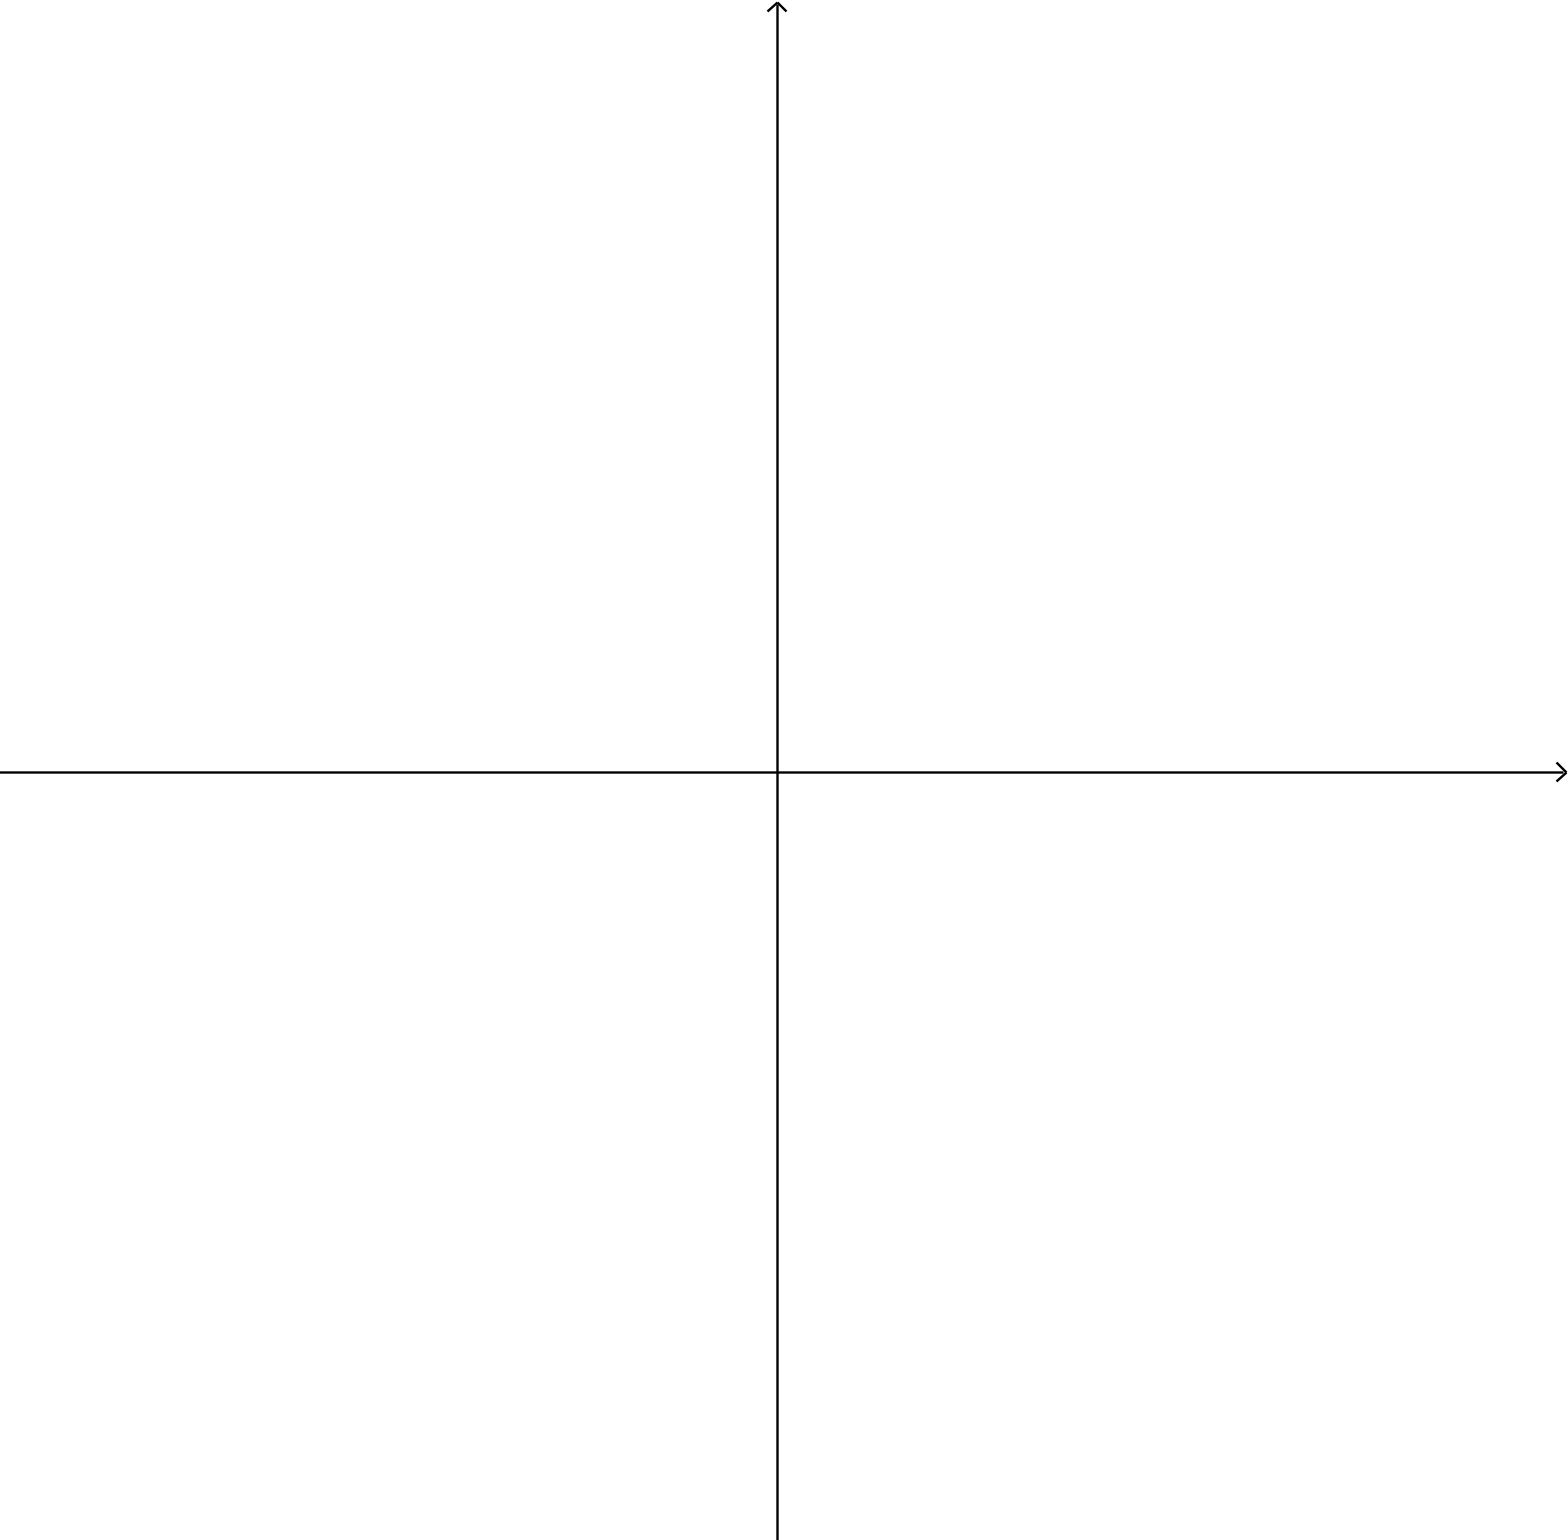
\includegraphics[width=0.9\textwidth]{66}
\end{minipage}
\begin{minipage}{0.45\textwidth}\centering
\(y=x^2+2x+3\)
\par\bigskip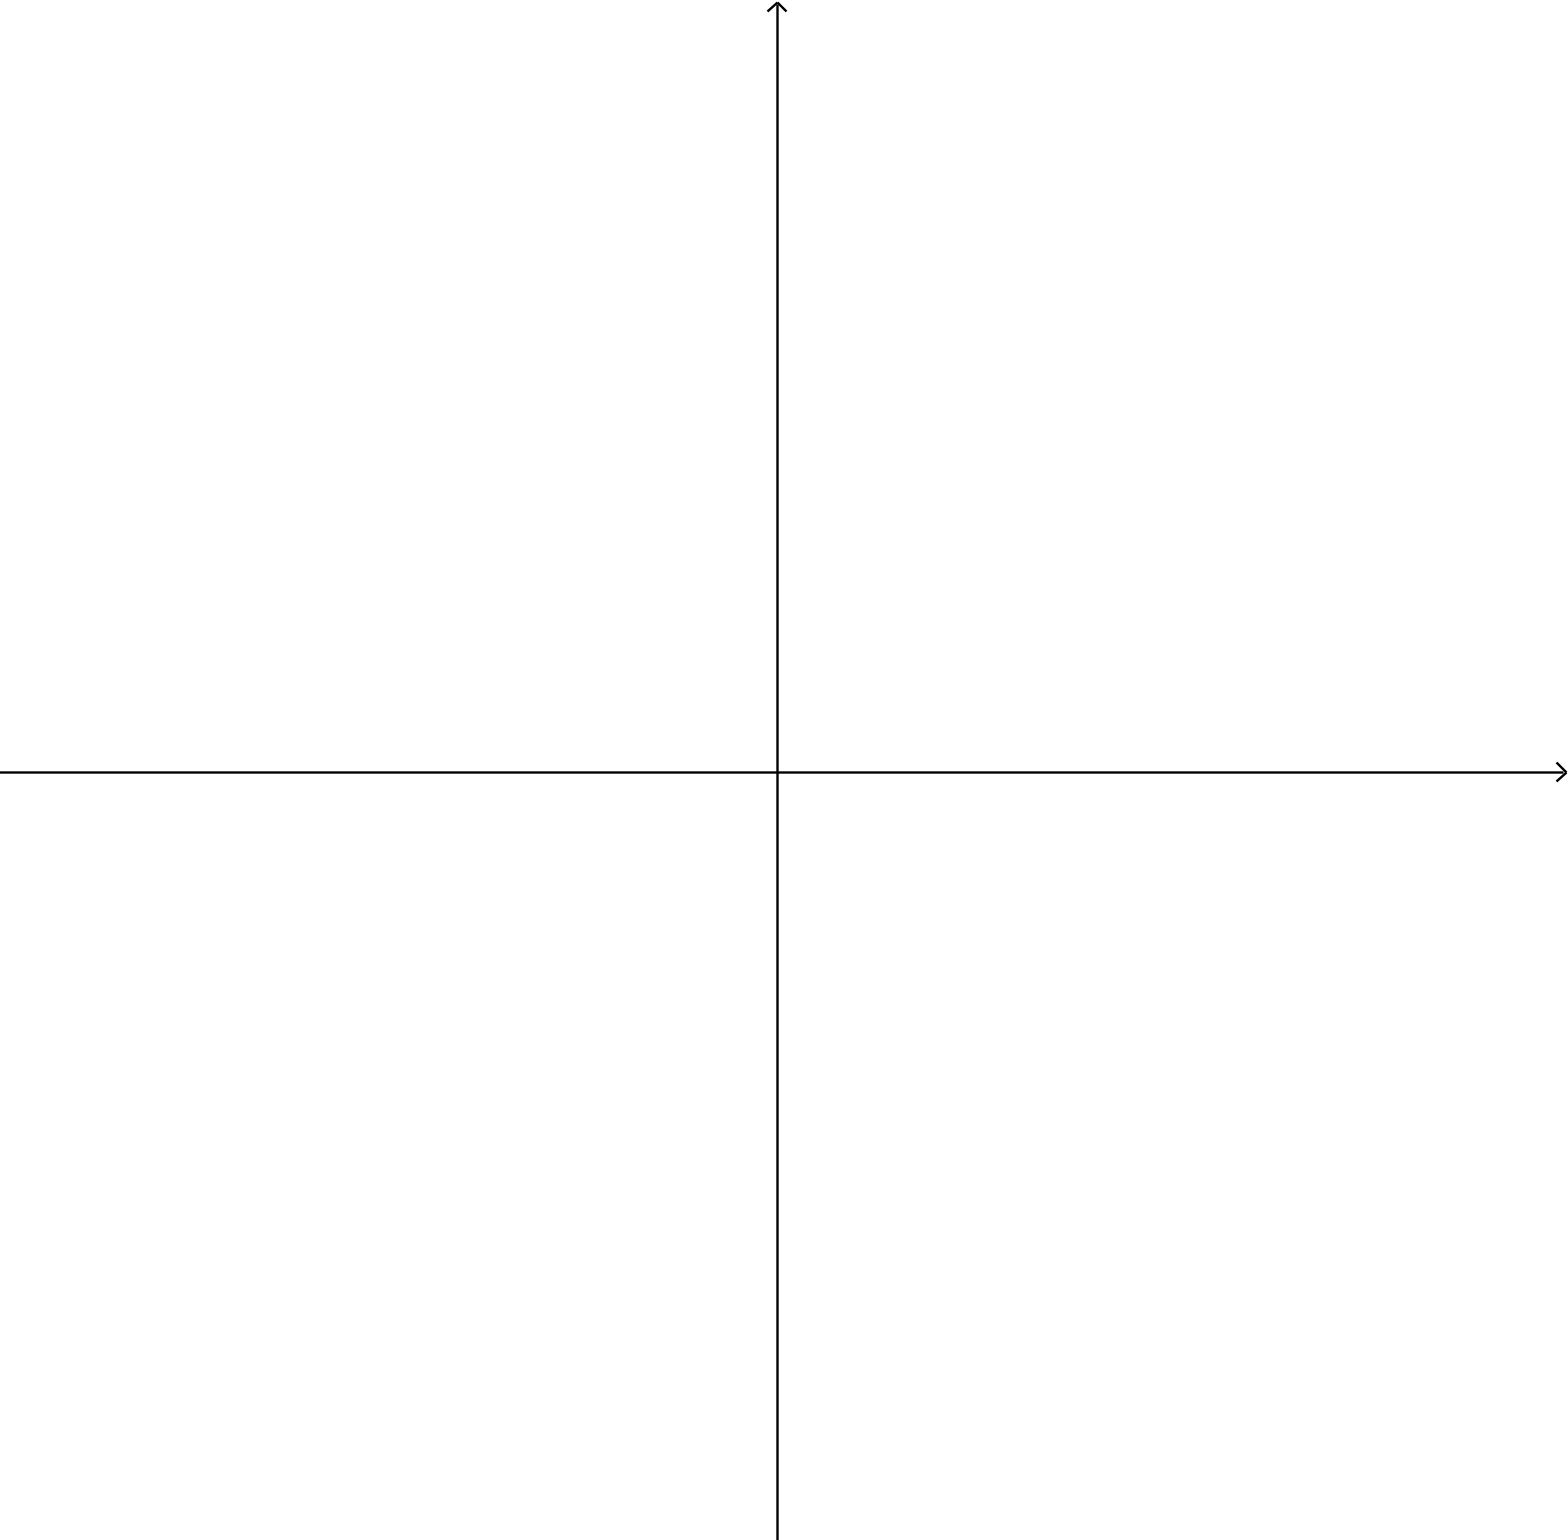
\includegraphics[width=0.9\textwidth]{66}
\end{minipage}\bigskip\bigskip\par
\begin{minipage}{0.45\textwidth}\centering
\(y=2x^2+8x\)
\par\bigskip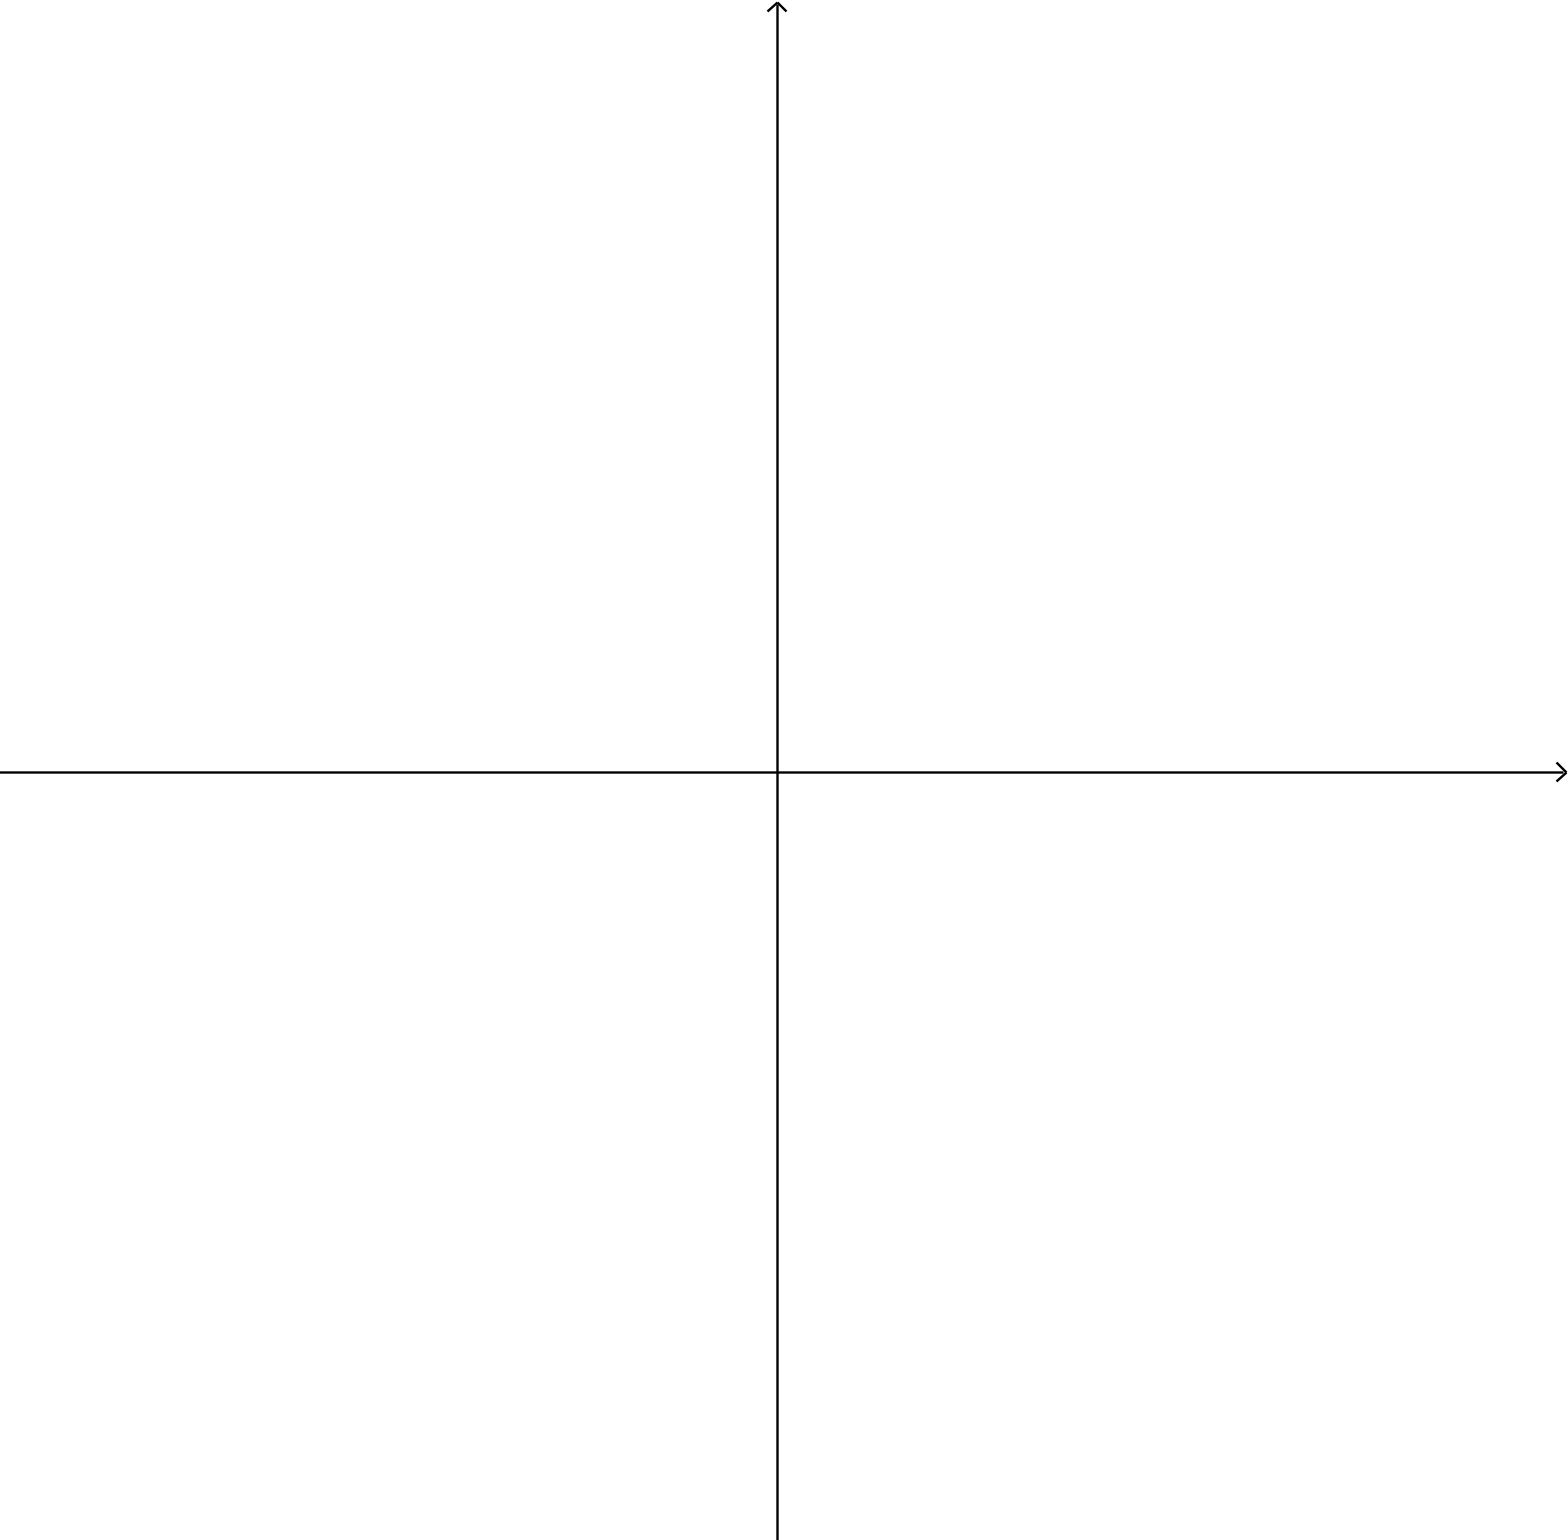
\includegraphics[width=0.9\textwidth]{66}
\end{minipage}
\begin{minipage}{0.45\textwidth}\centering
\(y=2x^2-4x-1\)
\par\bigskip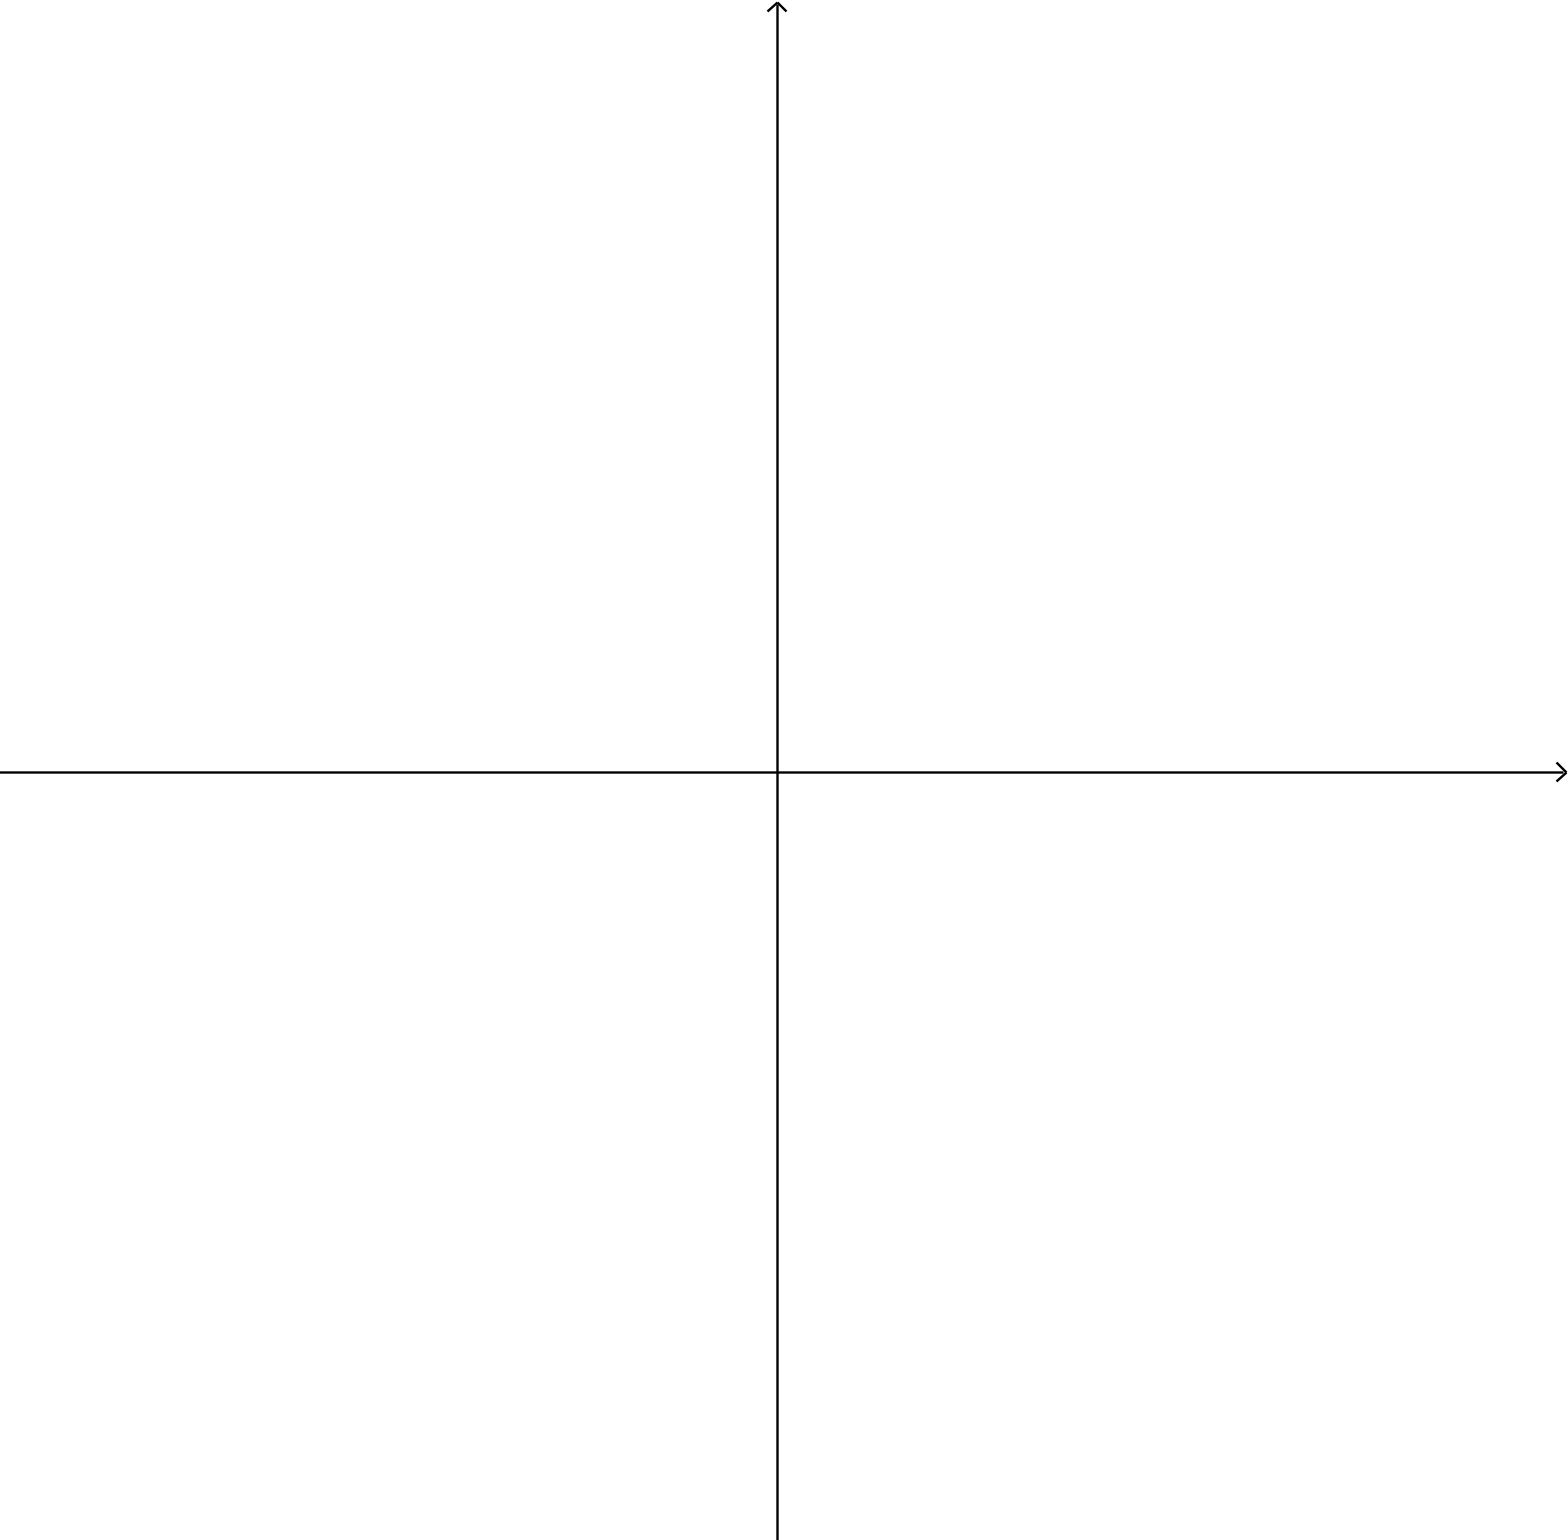
\includegraphics[width=0.9\textwidth]{66}
\end{minipage}\bigskip\bigskip\par

\clearpage
\begin{minipage}{0.45\textwidth}\centering
\(y=3x^2-18x\)
\par\bigskip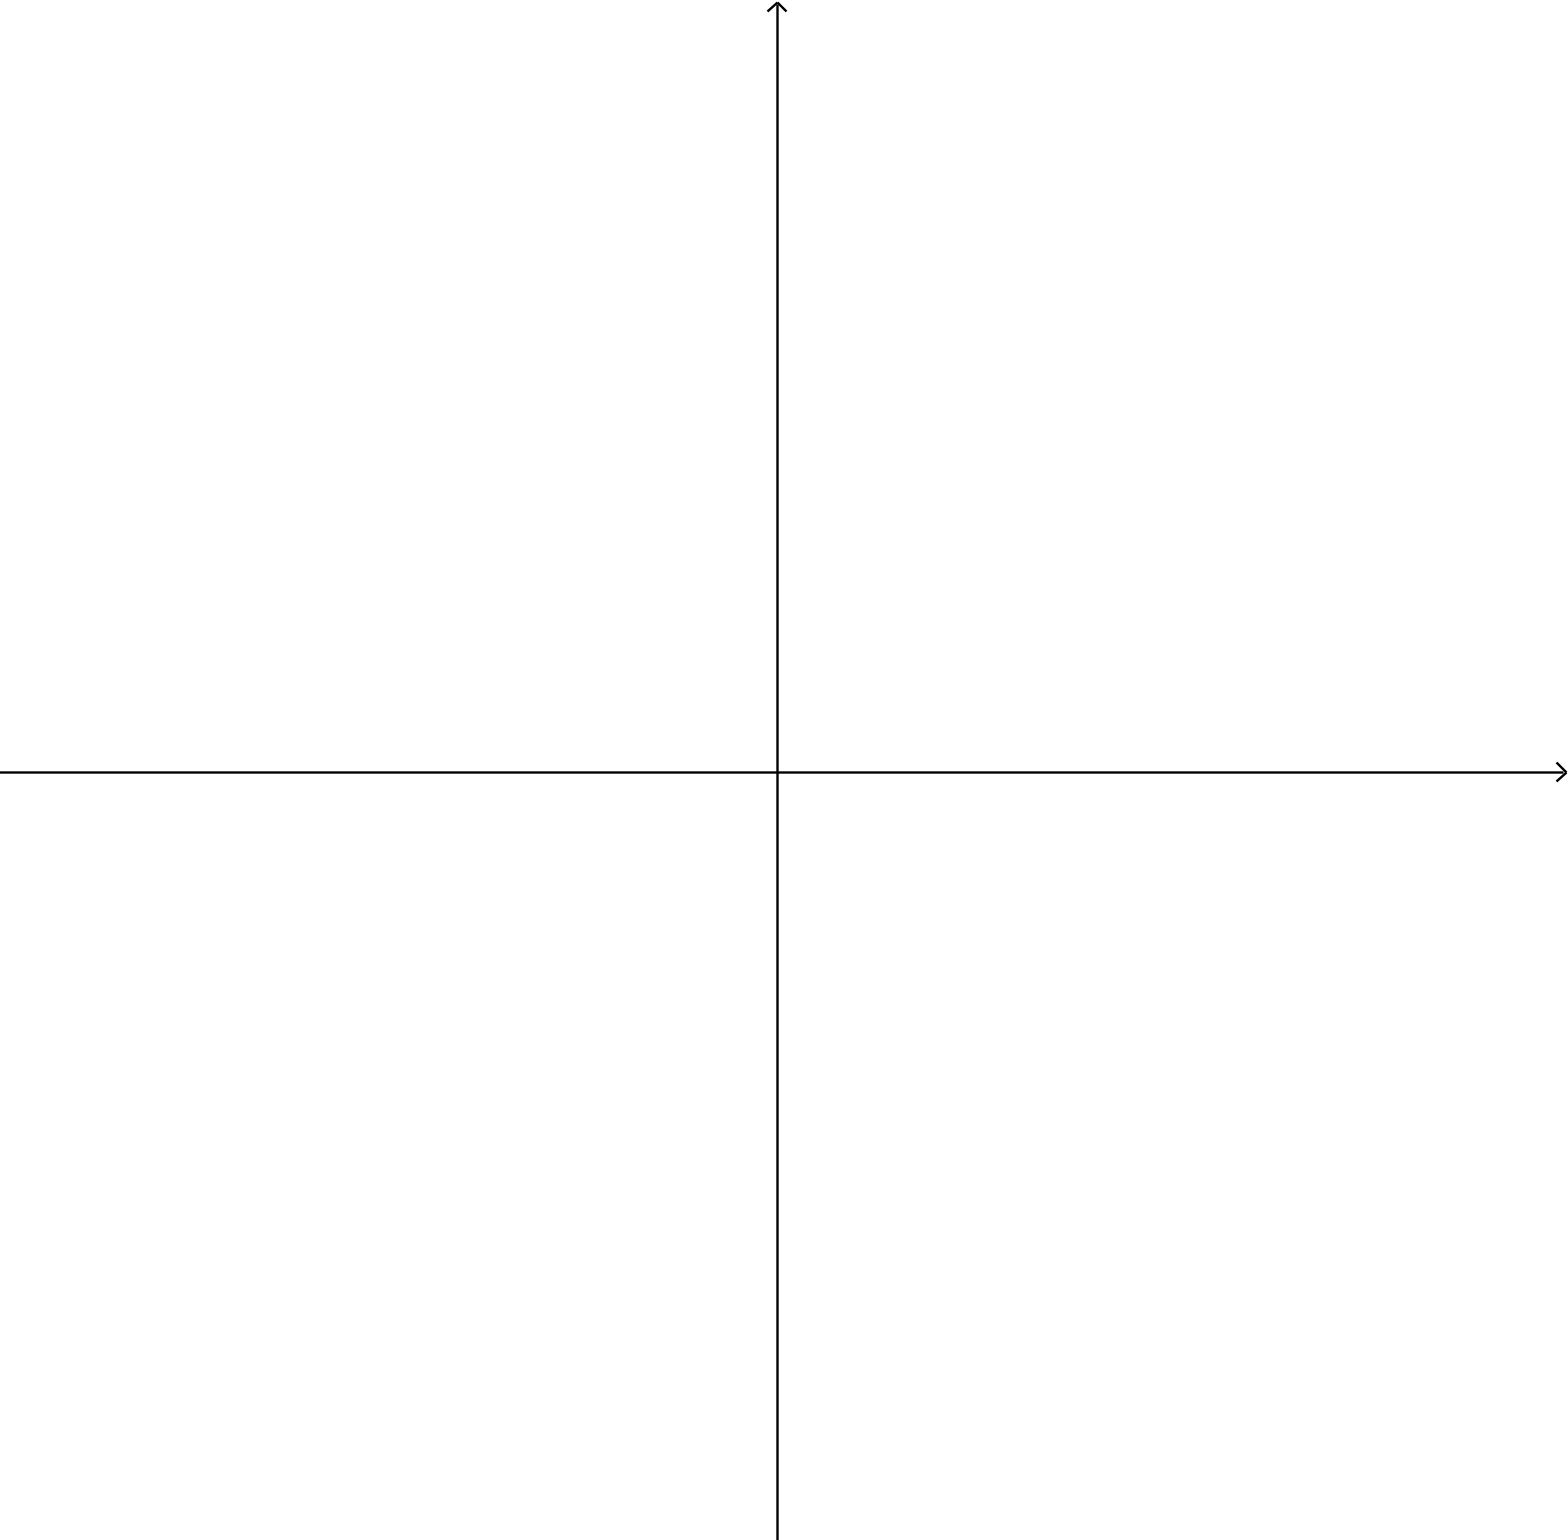
\includegraphics[width=0.9\textwidth]{66}
\end{minipage}
\begin{minipage}{0.45\textwidth}\centering
\(y=4x^2-8x-1\)
\par\bigskip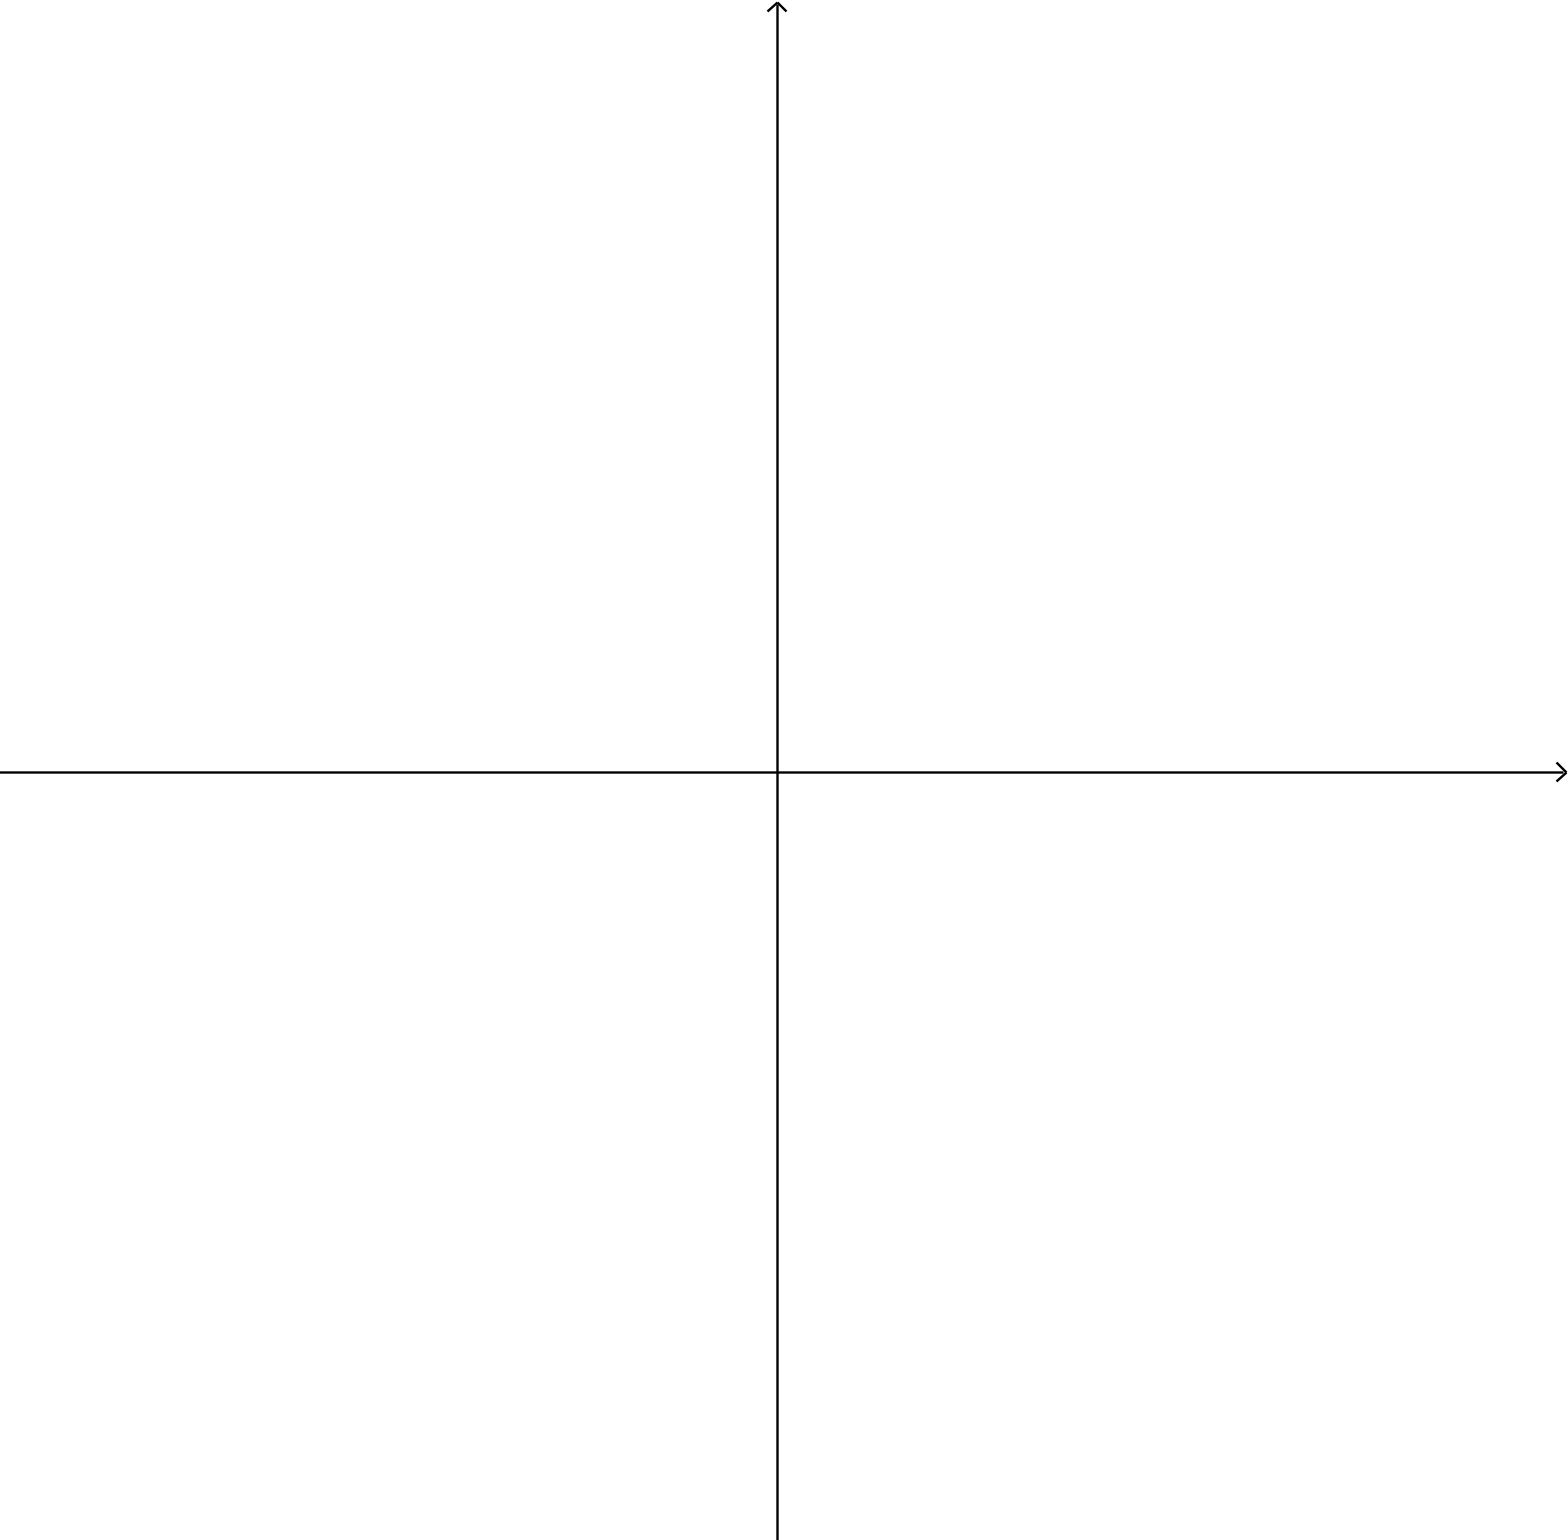
\includegraphics[width=0.9\textwidth]{66}
\end{minipage}\bigskip\bigskip\par
\begin{minipage}{0.45\textwidth}\centering
\(y=x^2-3x+3\)
\par\bigskip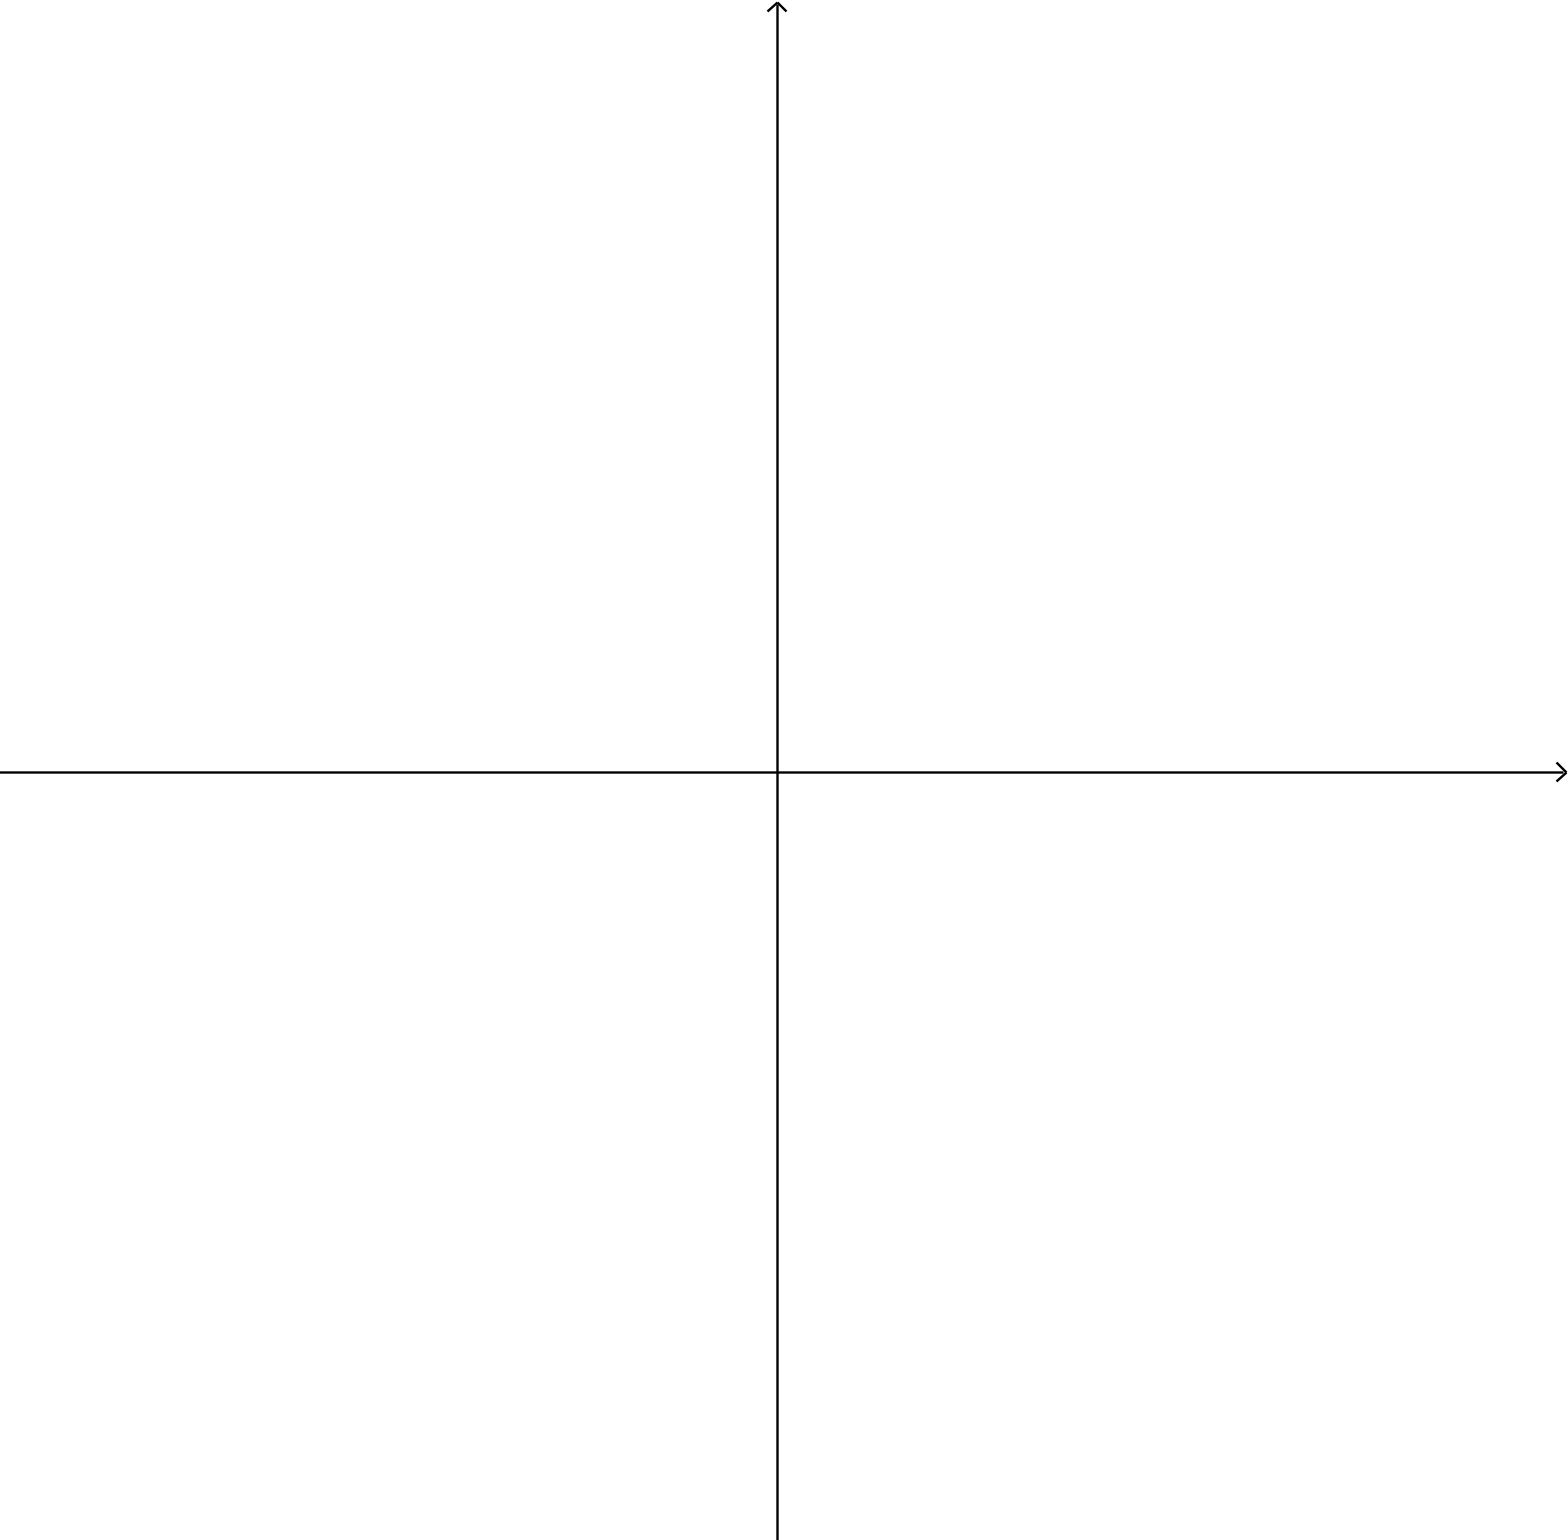
\includegraphics[width=0.9\textwidth]{66}
\end{minipage}
\begin{minipage}{0.45\textwidth}\centering
\(y=x^2+x+1\)
\par\bigskip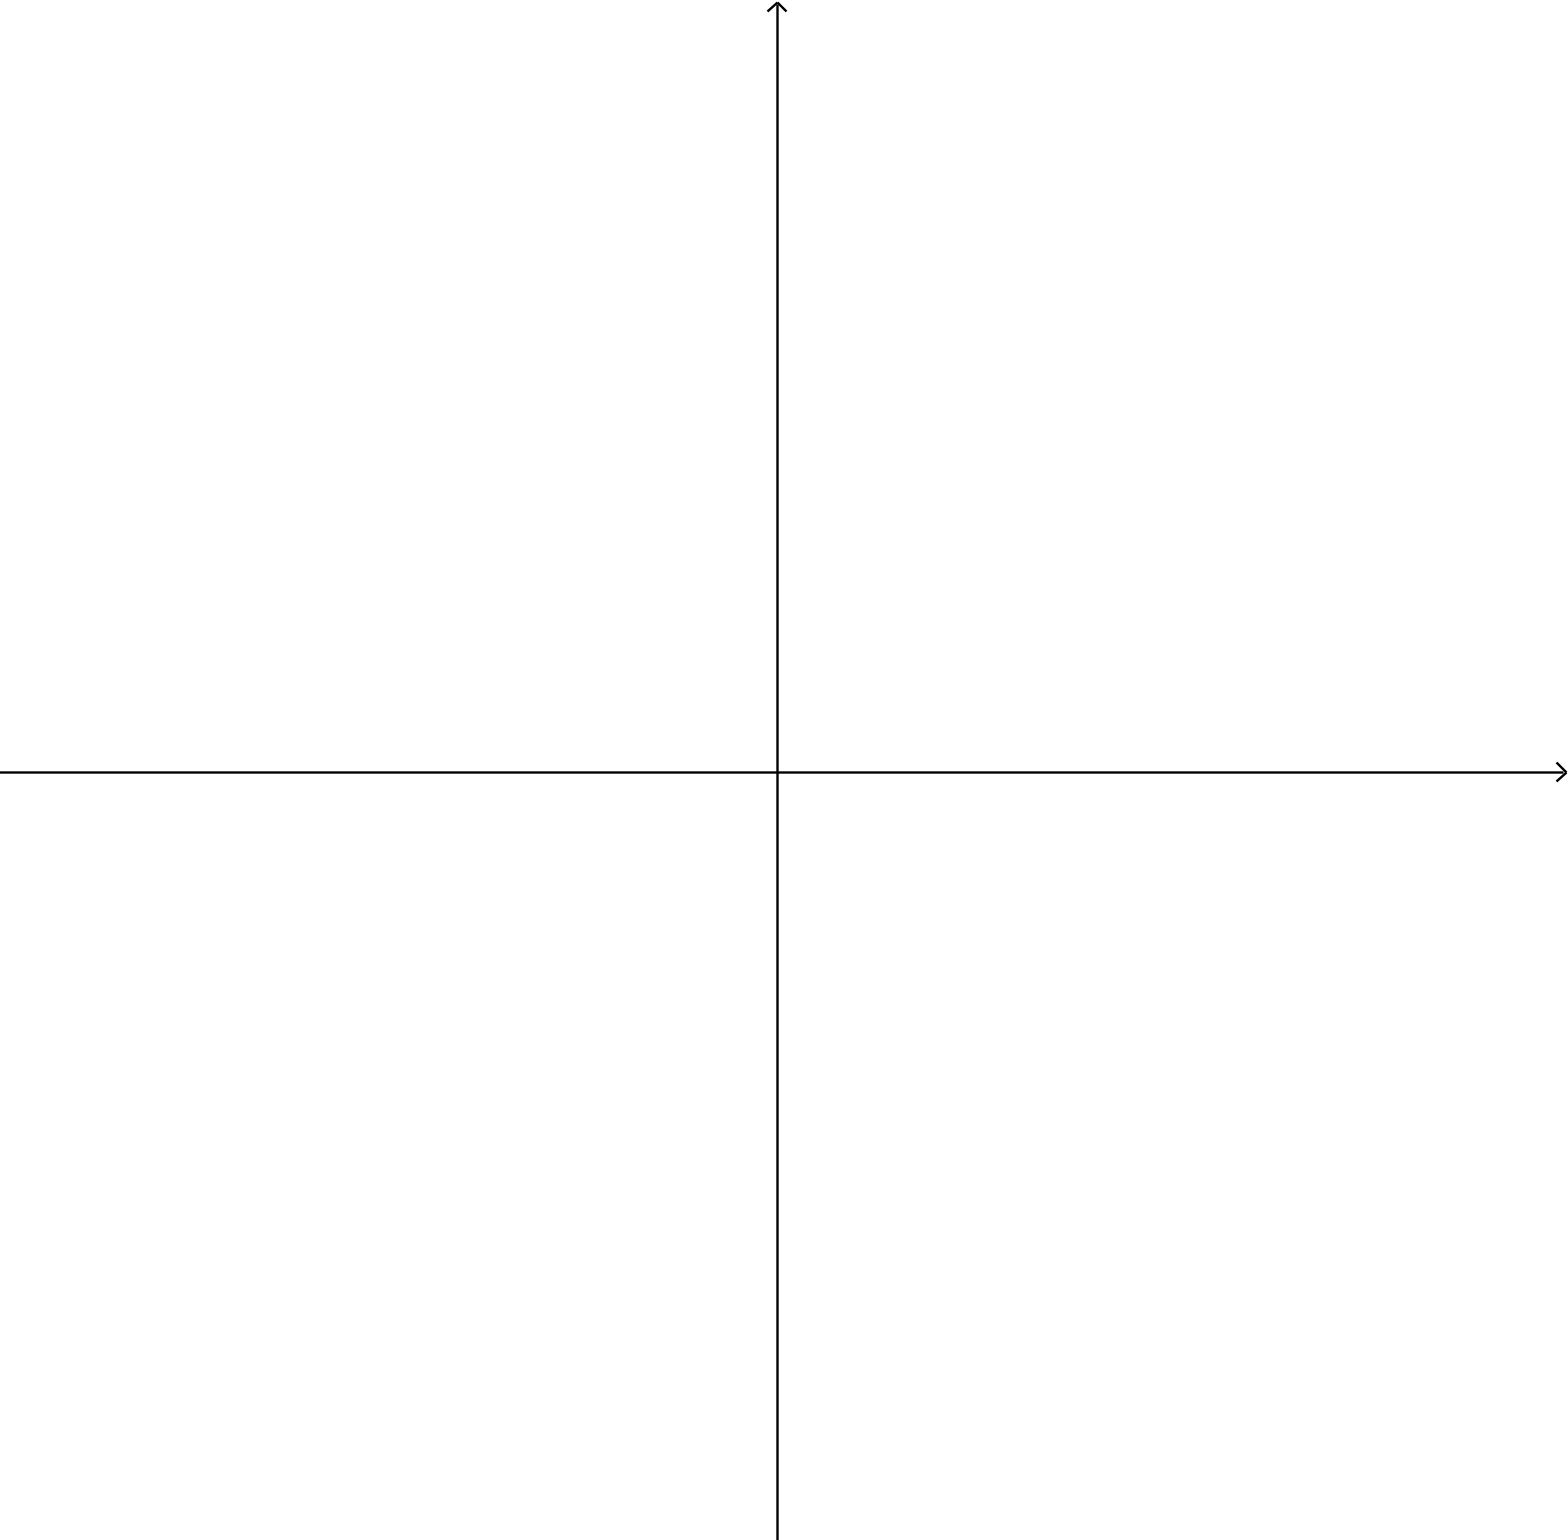
\includegraphics[width=0.9\textwidth]{66}
\end{minipage}\bigskip\bigskip\par
\begin{minipage}{0.45\textwidth}\centering
\(y=2x^2+3x-2\)
\par\bigskip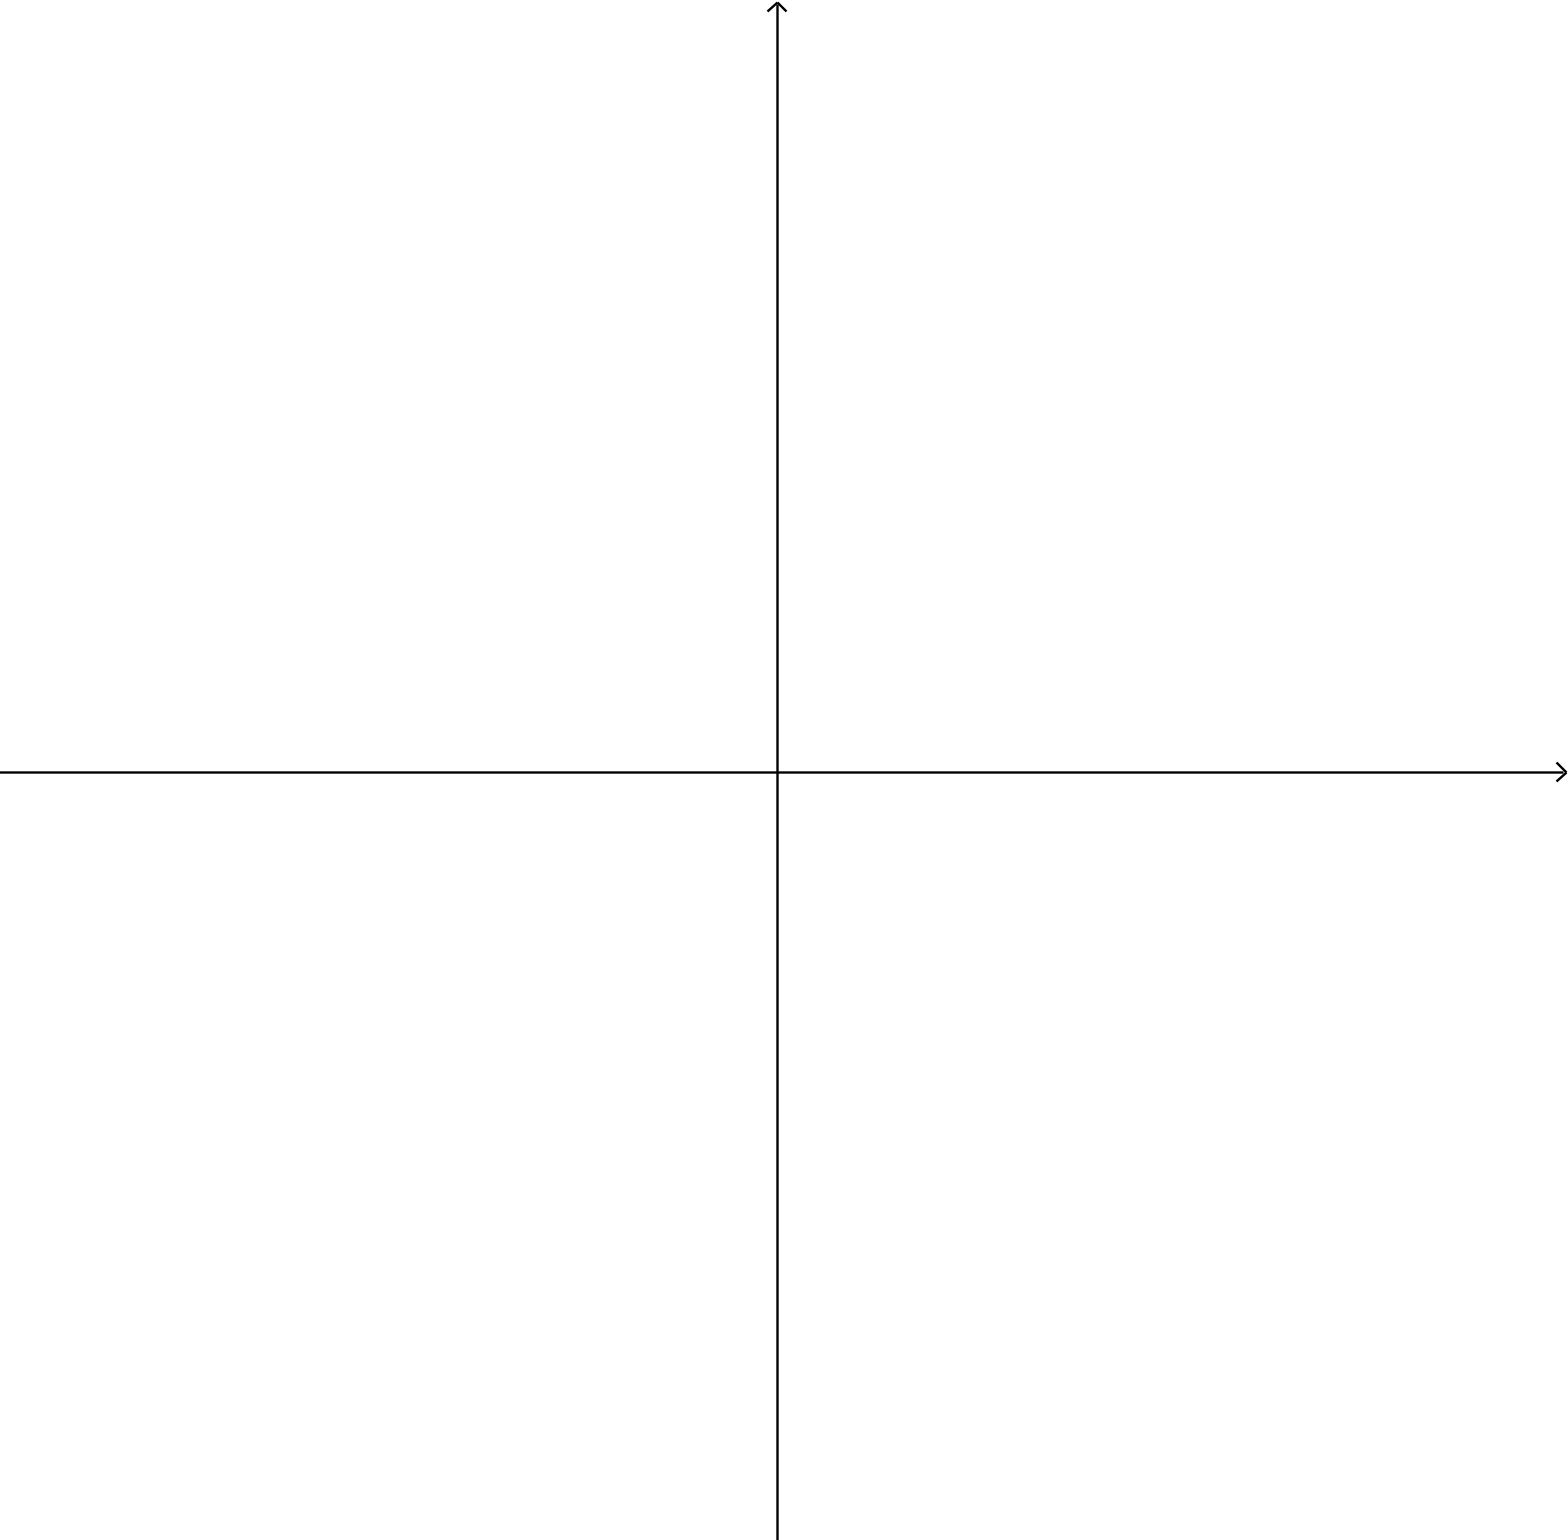
\includegraphics[width=0.9\textwidth]{66}
\end{minipage}
\begin{minipage}{0.45\textwidth}\centering
\(y=3x^2-9x+1\)
\par\bigskip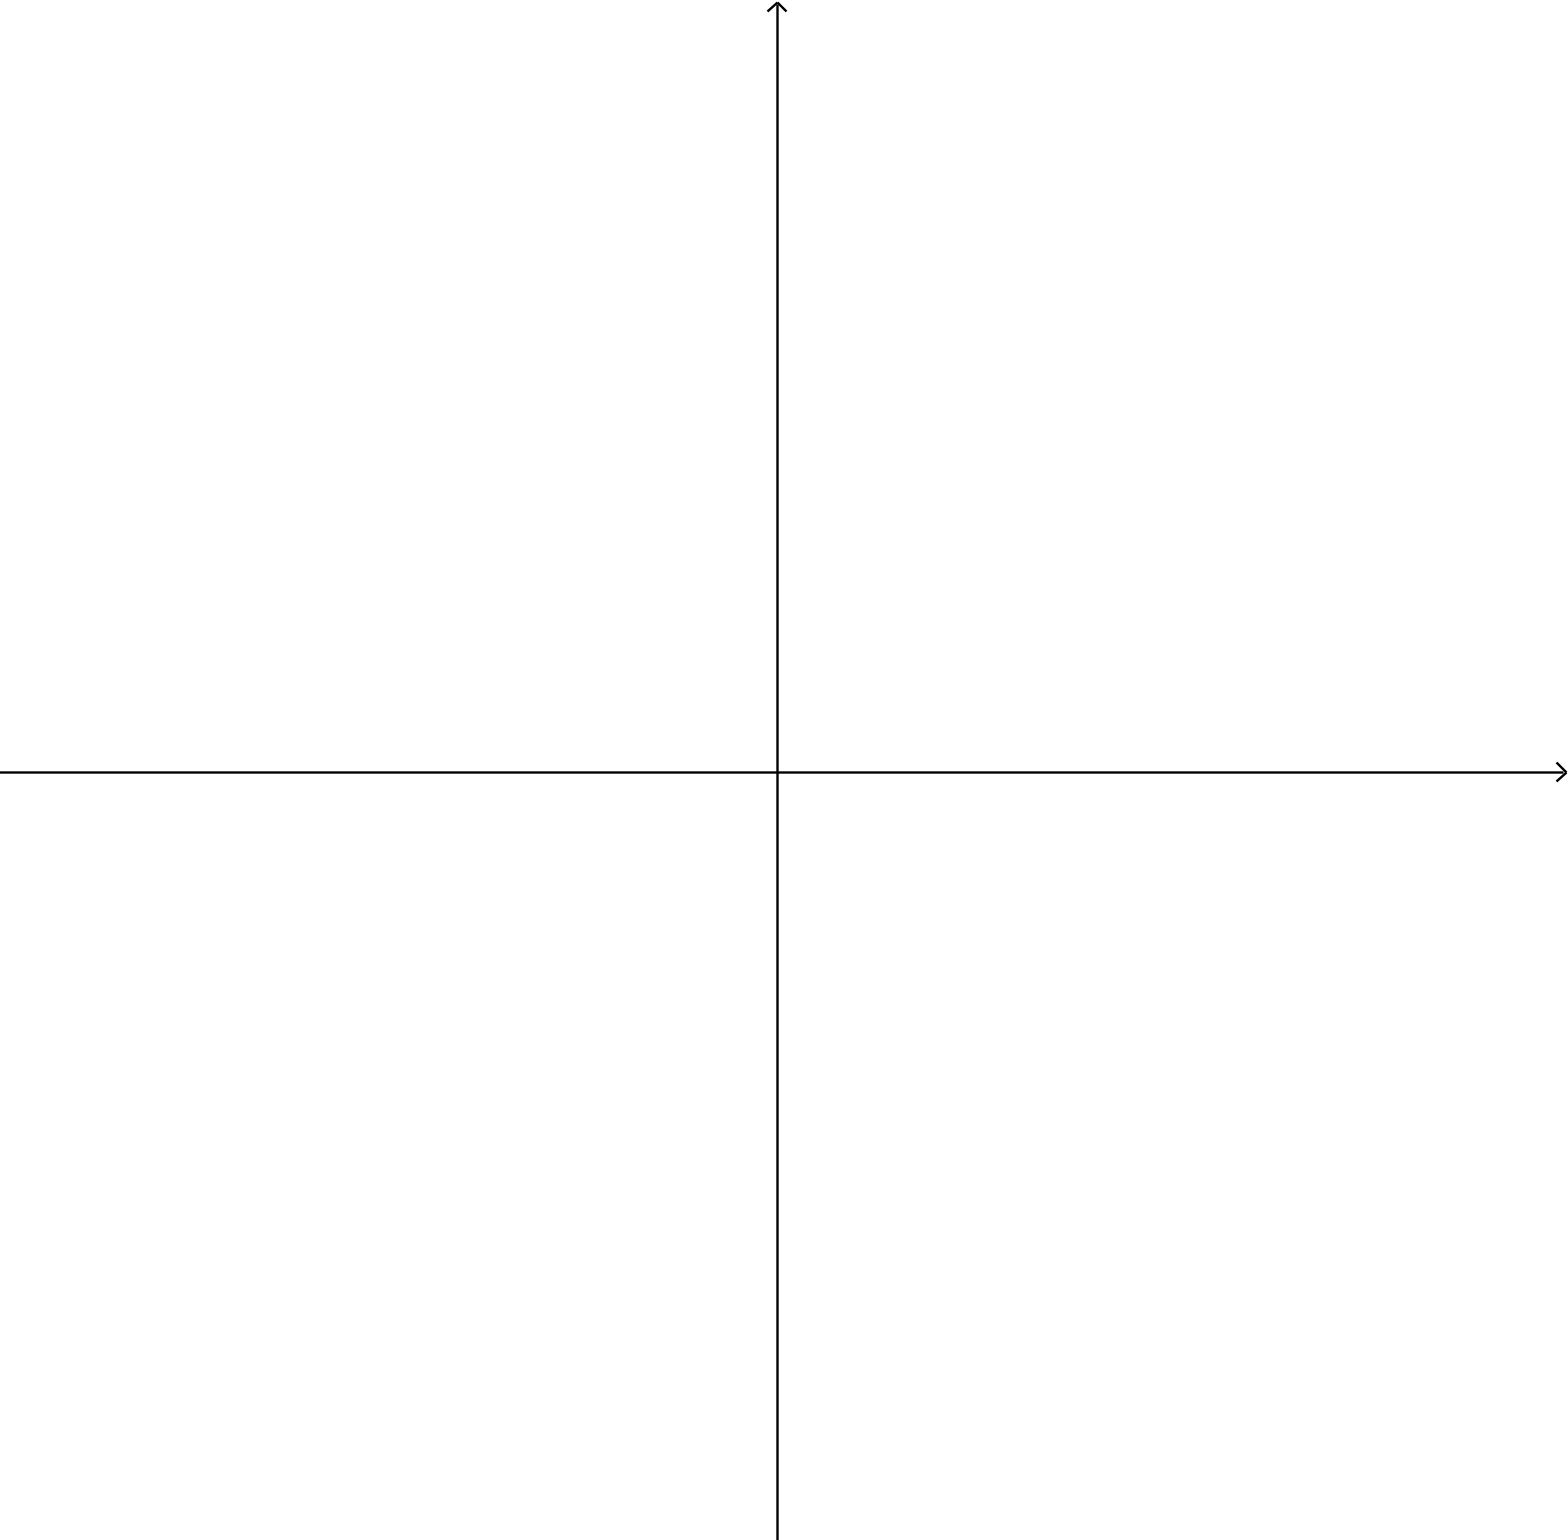
\includegraphics[width=0.9\textwidth]{66}
\end{minipage}\bigskip\bigskip\par

\clearpage
\begin{minipage}{0.45\textwidth}\centering
\(y=-x^2+2x\)
\par\bigskip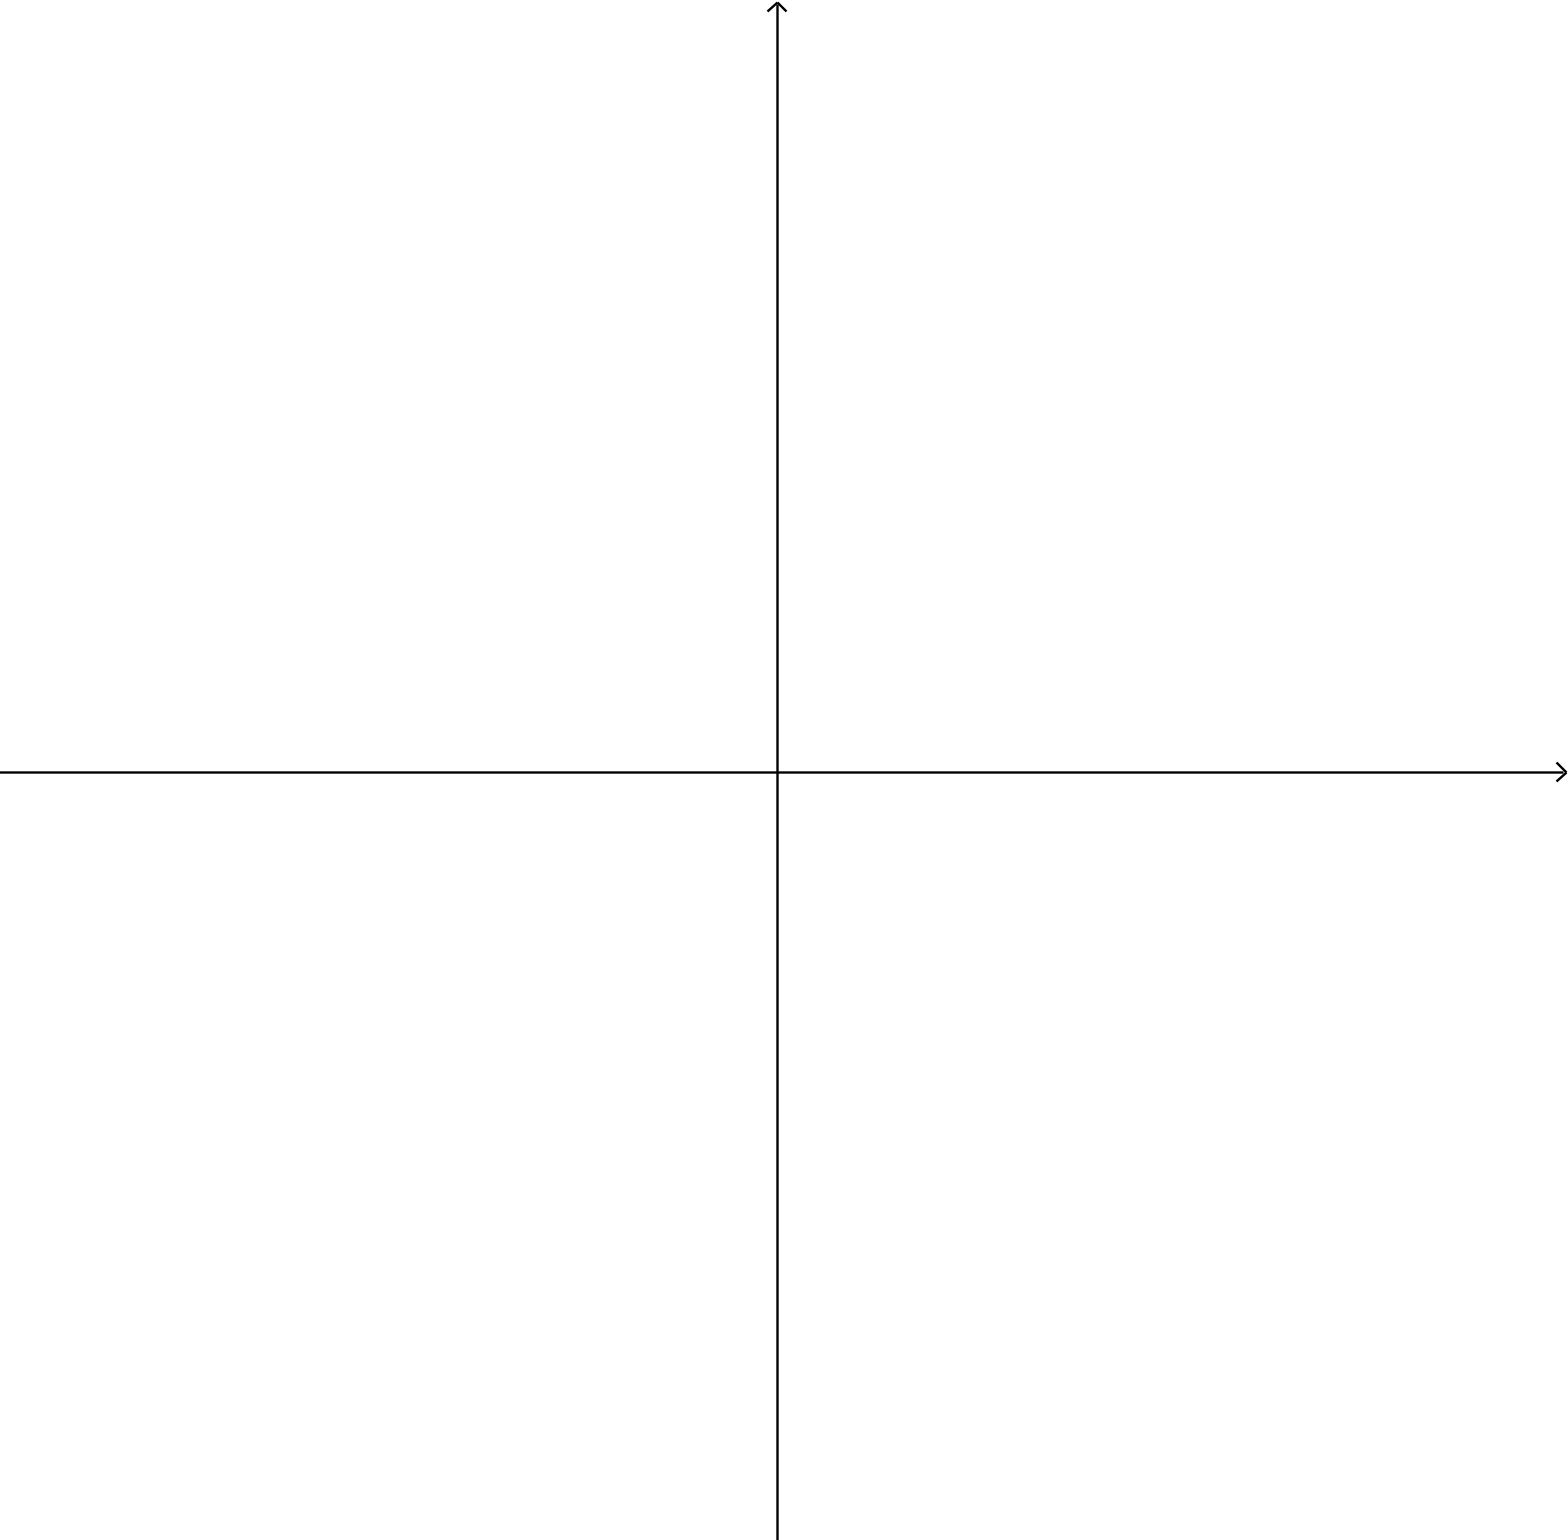
\includegraphics[width=0.9\textwidth]{66}
\end{minipage}
\begin{minipage}{0.45\textwidth}\centering
\(y=-x^2-4x-3\)
\par\bigskip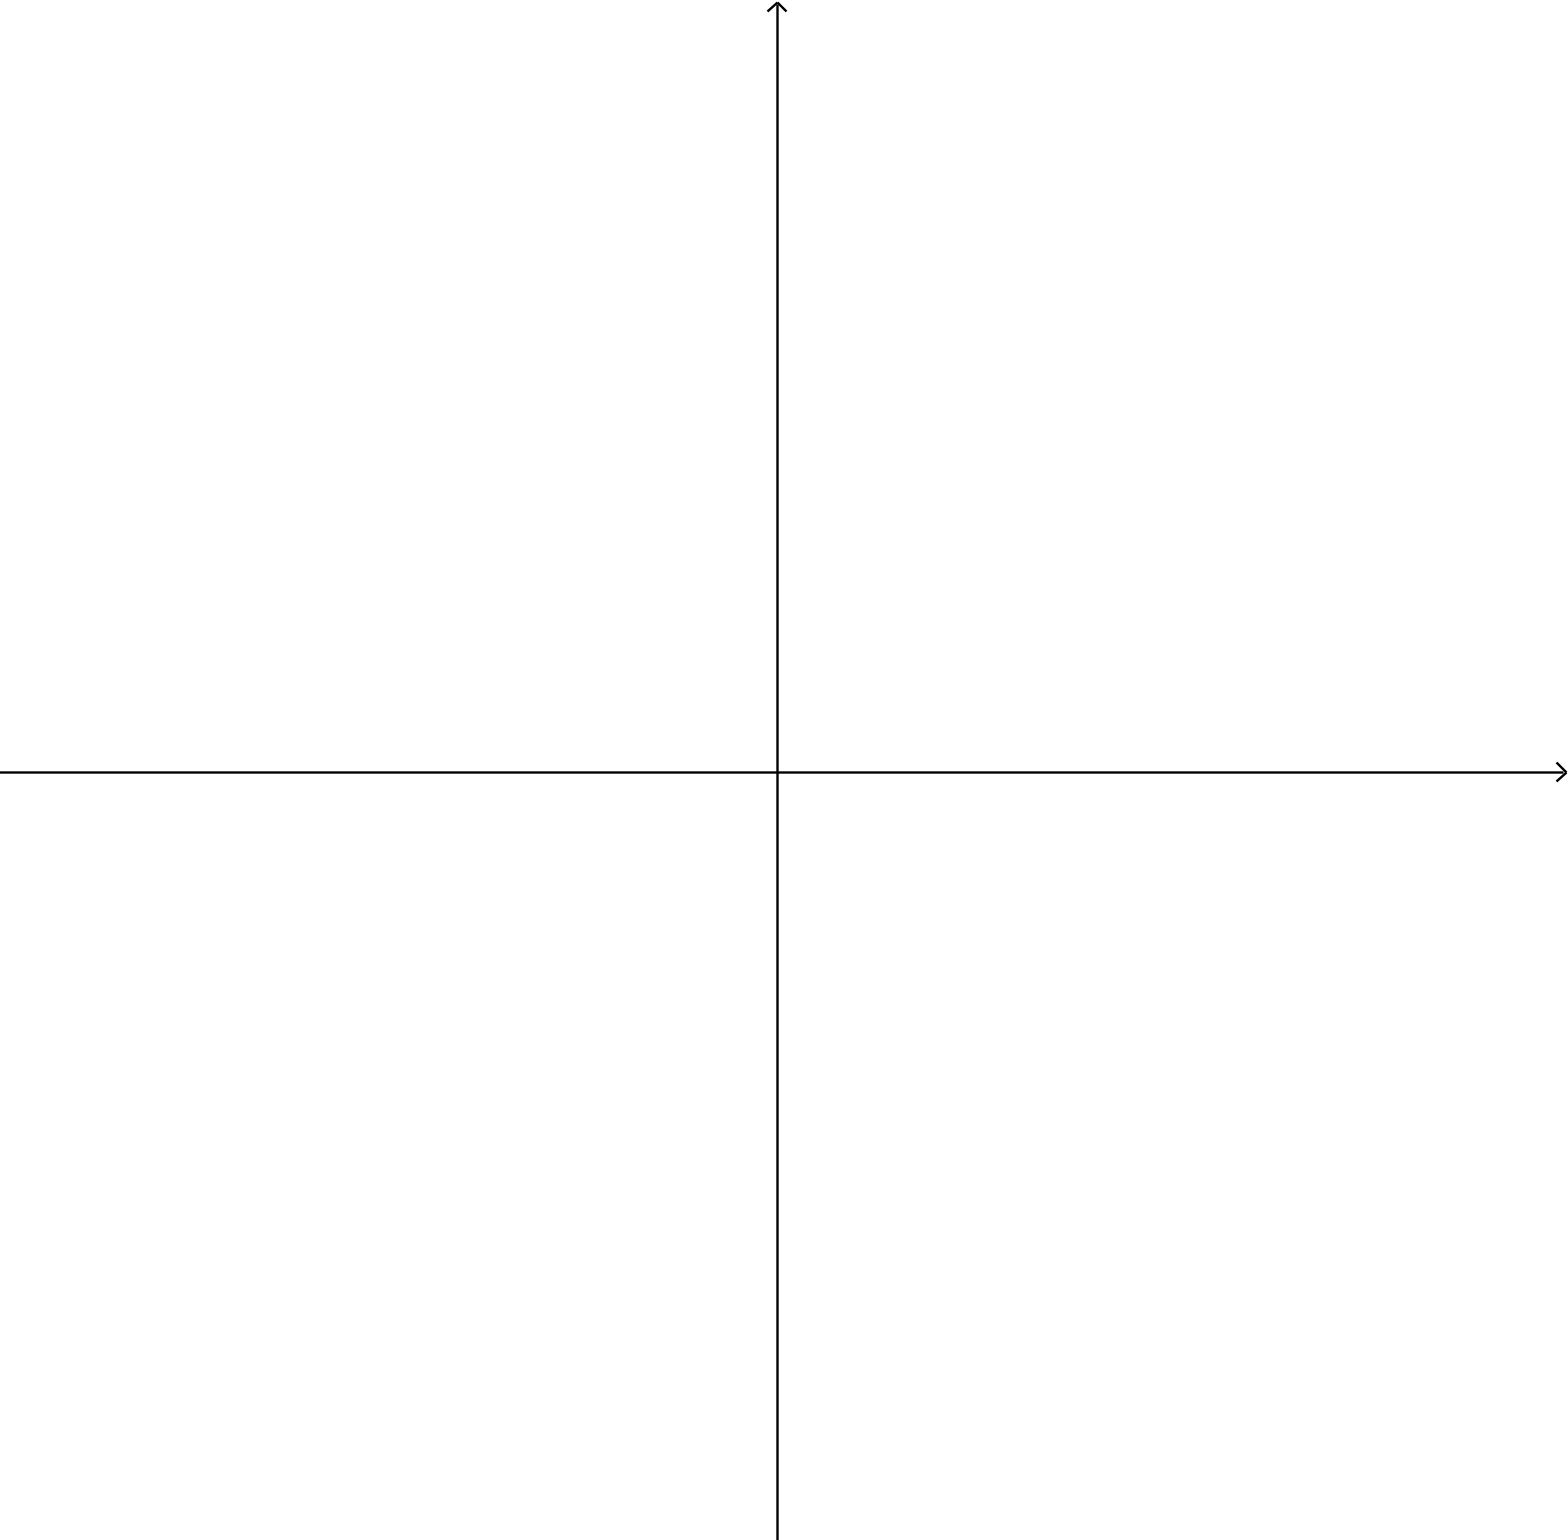
\includegraphics[width=0.9\textwidth]{66}
\end{minipage}\bigskip\bigskip\par
\begin{minipage}{0.45\textwidth}\centering
\(y=\frac12x^2-x+2\)
\par\bigskip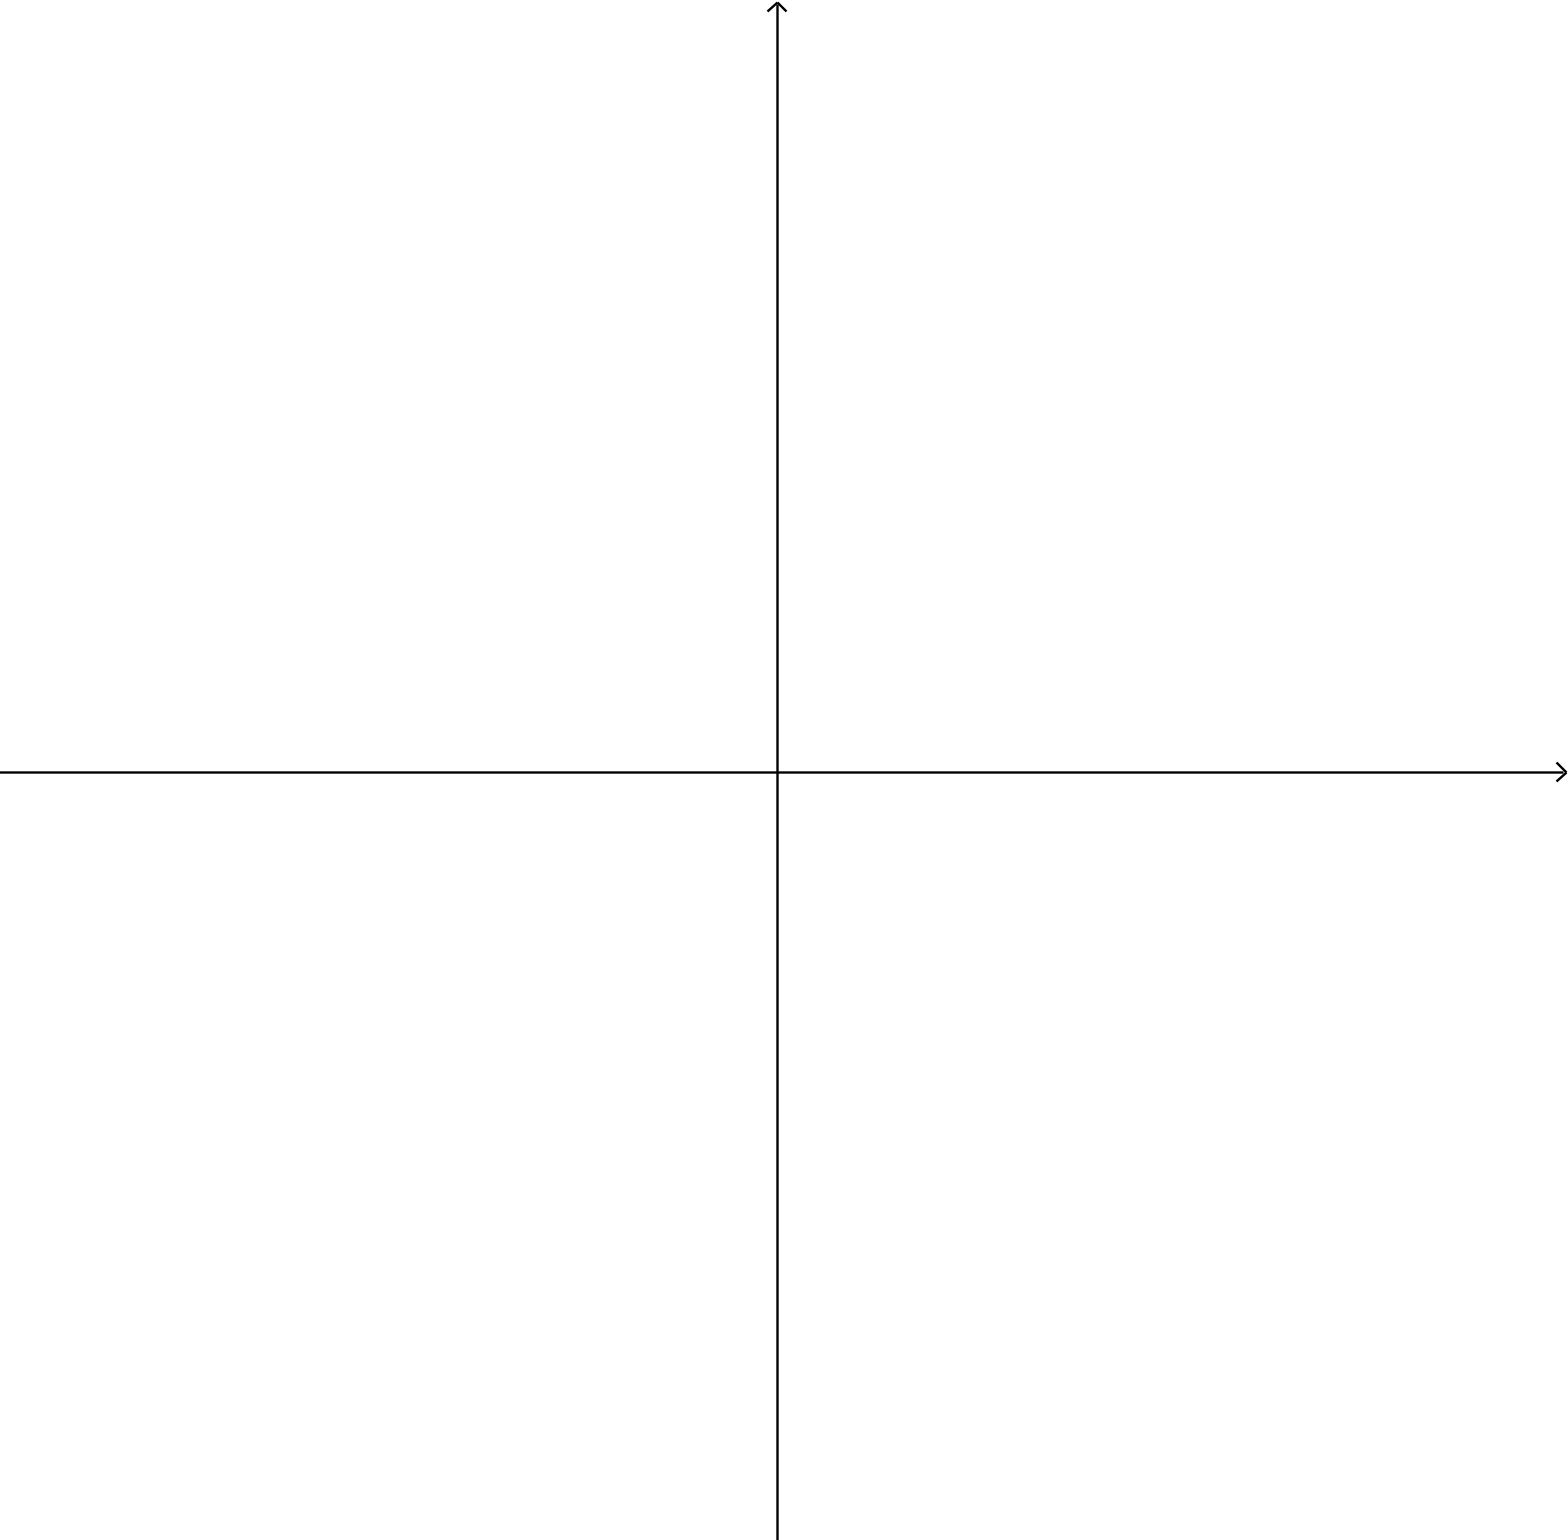
\includegraphics[width=0.9\textwidth]{66}
\end{minipage}
\begin{minipage}{0.45\textwidth}\centering
\(y=-\frac12x^2+3x-2\)
\par\bigskip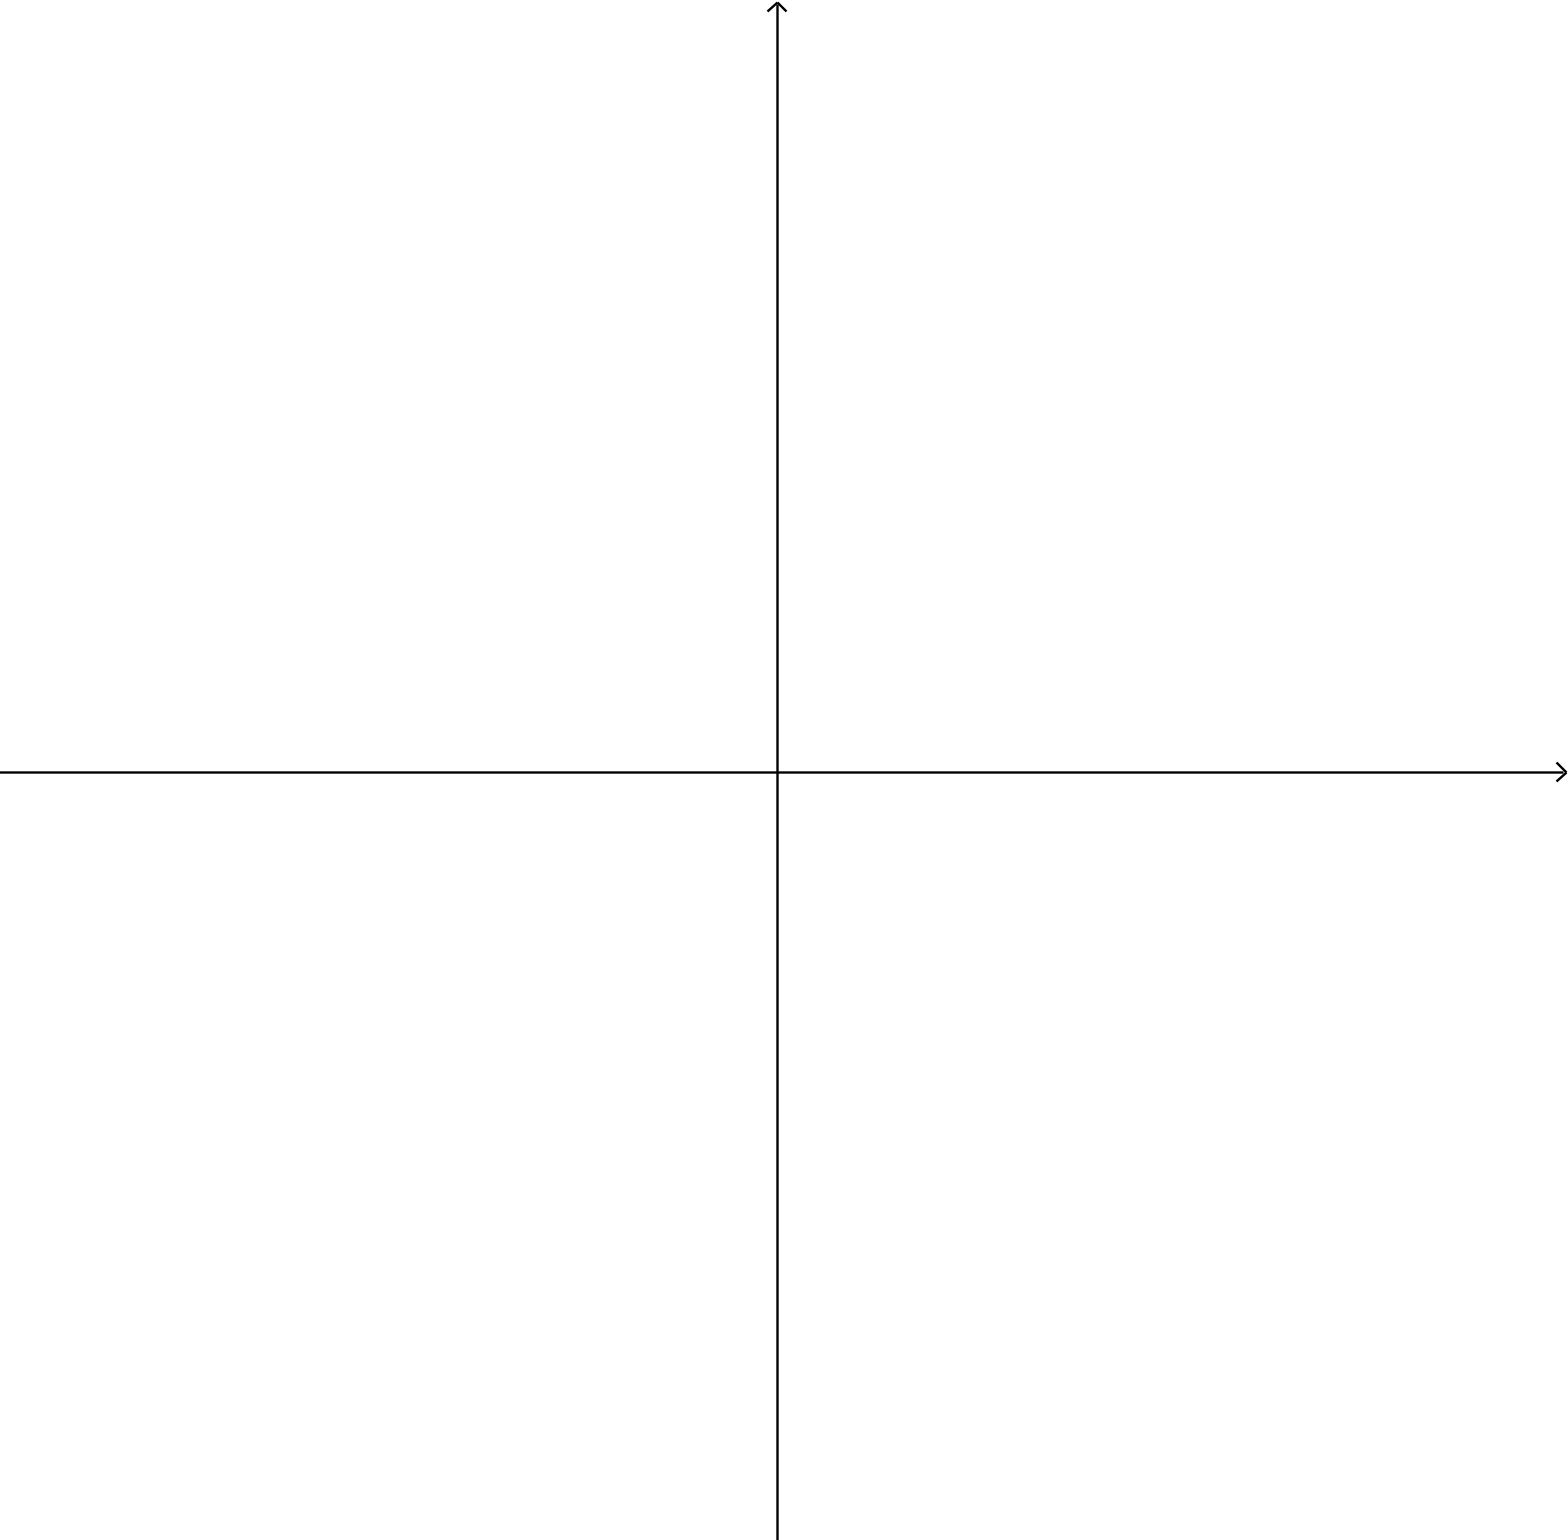
\includegraphics[width=0.9\textwidth]{66}
\end{minipage}\bigskip\bigskip\par
\begin{minipage}{0.45\textwidth}\centering
\(y=-\frac16x^2+\frac13x+\frac12\)
\par\bigskip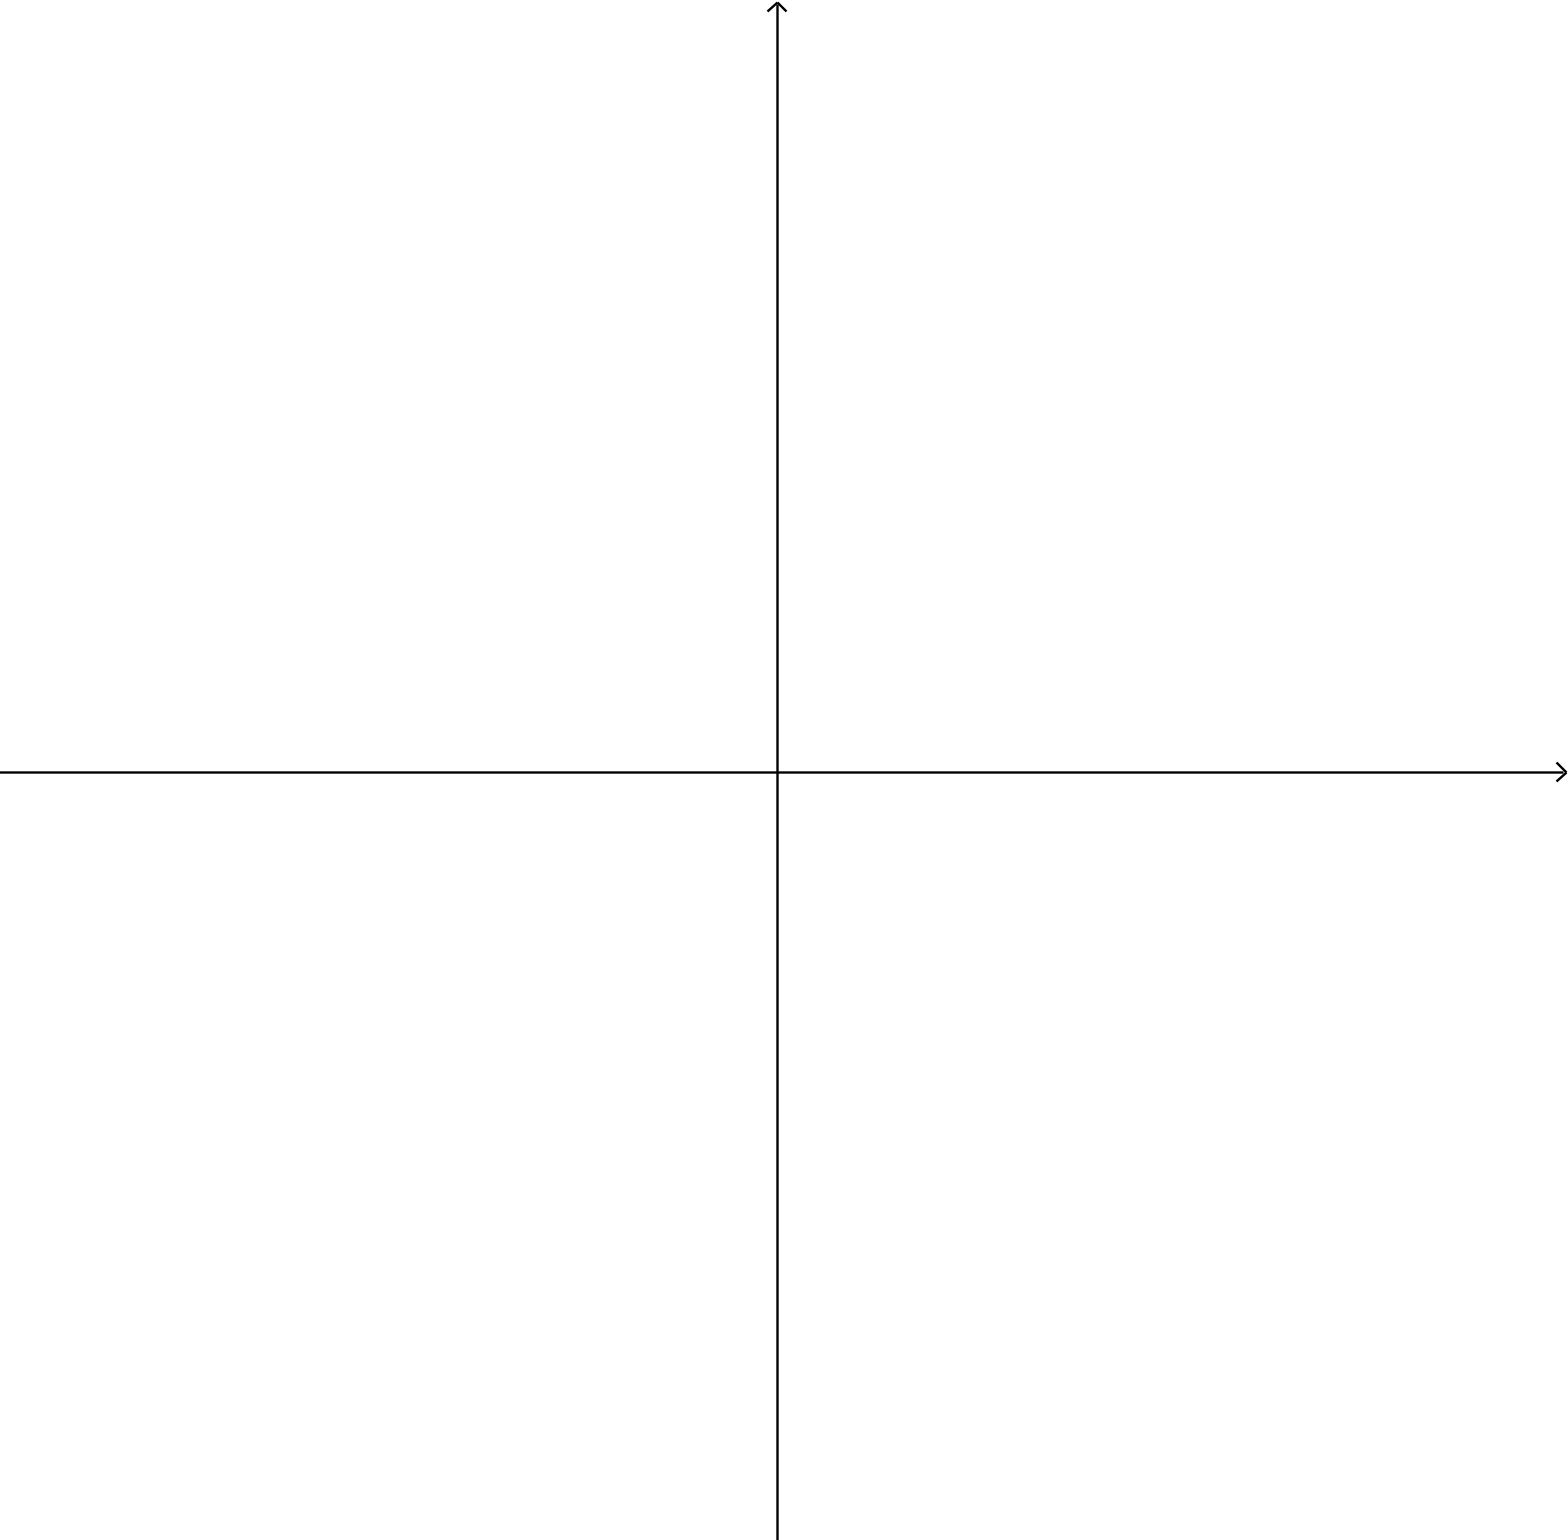
\includegraphics[width=0.9\textwidth]{66}
\end{minipage}
\begin{minipage}{0.45\textwidth}\centering
\(y=\frac13x^2-2x\)
\par\bigskip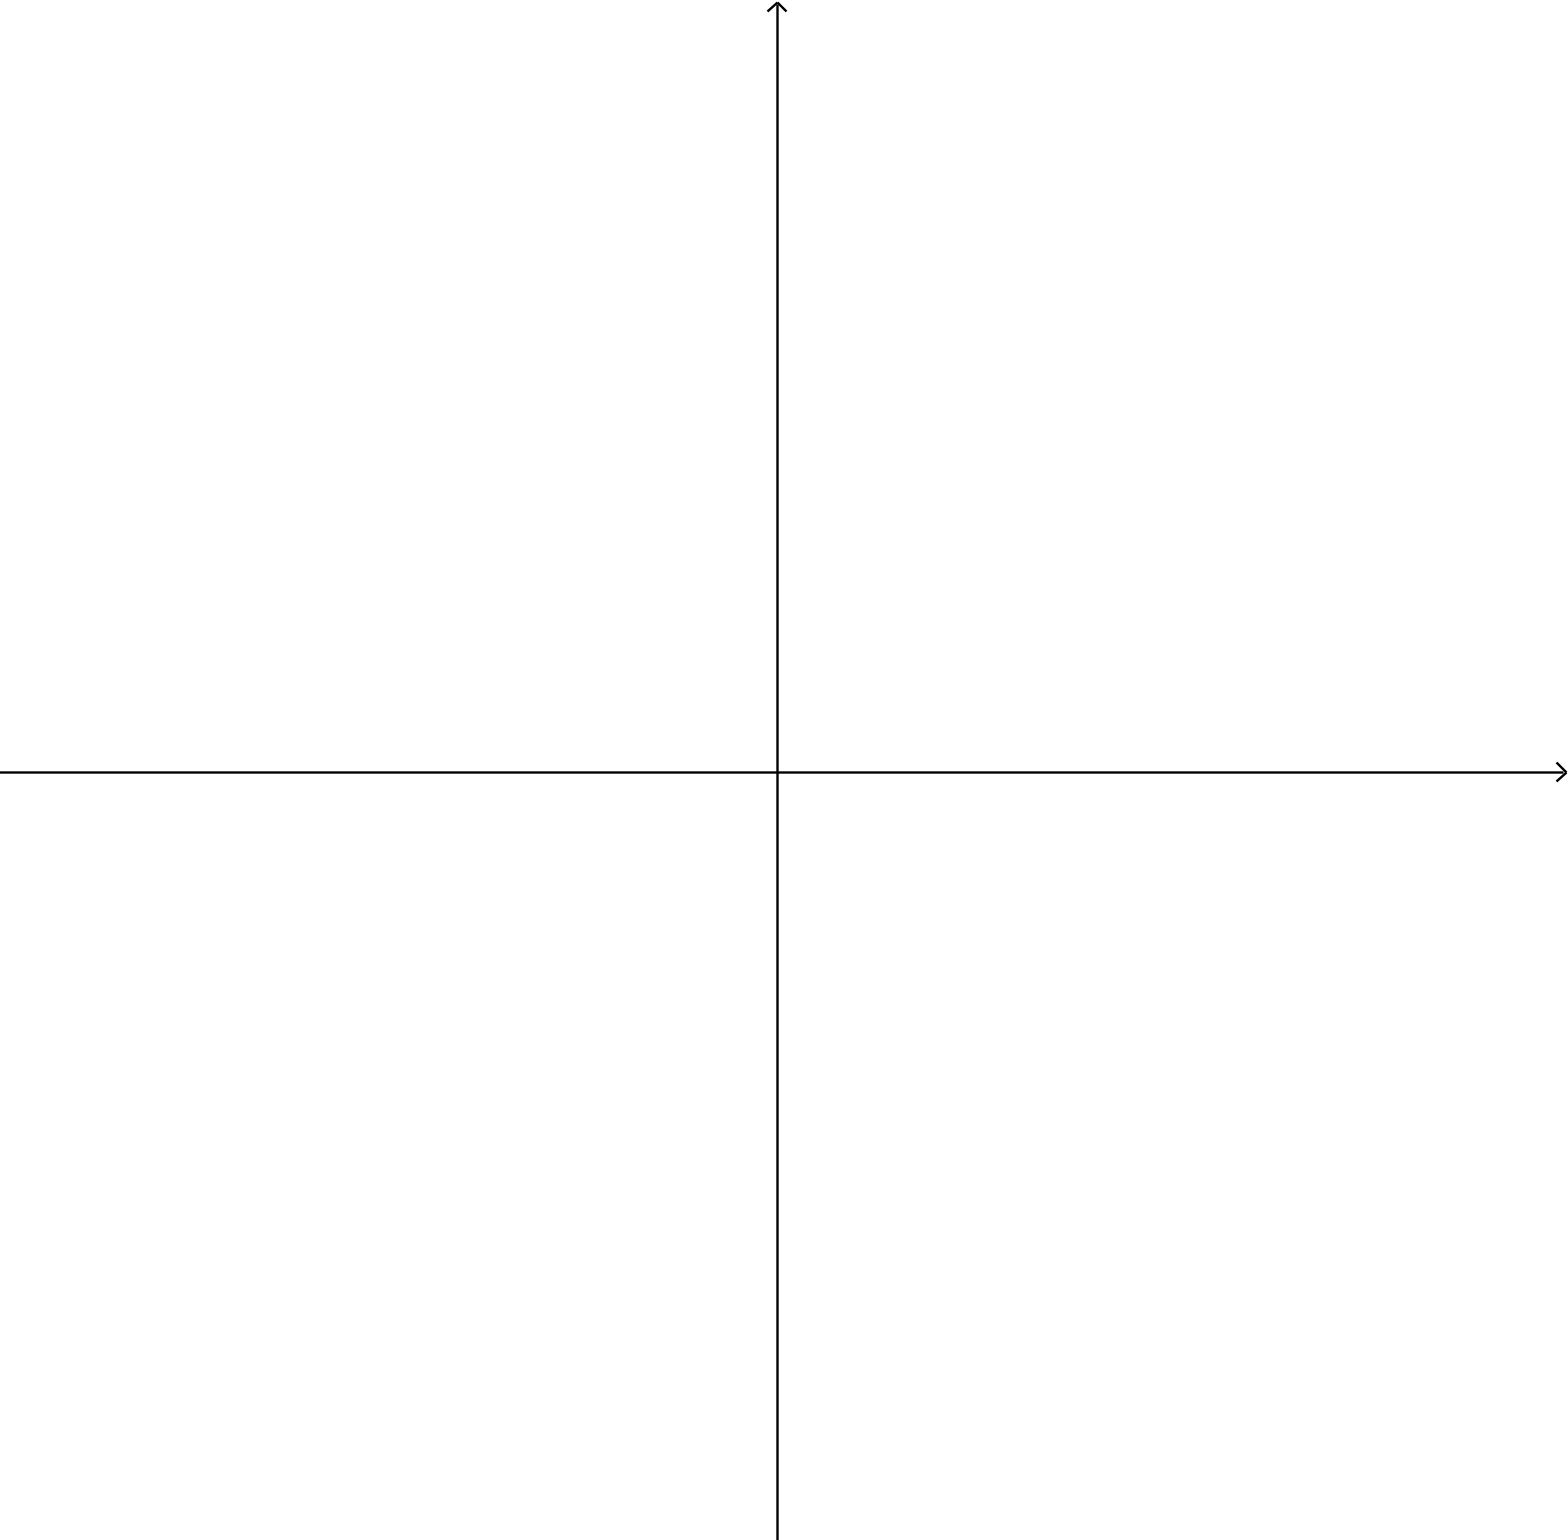
\includegraphics[width=0.9\textwidth]{66}
\end{minipage}\bigskip\bigskip\par

\end{document}